\documentclass[12pt]{article}
\usepackage[utf8]{inputenc}
\usepackage{amsmath}
\usepackage{graphicx}
\usepackage{dsfont}
\usepackage{amsthm}
\usepackage{amssymb}
\usepackage{graphicx}
\usepackage{commath}
\usepackage{tensor}
\usepackage{mathtools}
\usepackage{tikz}
\usetikzlibrary{decorations.markings}
\usepackage{physics}
\usepackage{hyperref}
\usepackage{tcolorbox}
\usepackage{pgfplots}
\pgfplotsset{compat=1.6}
    \usetikzlibrary{
        decorations.markings, 
    }
    \tikzset{
        fleche/.style args={#1:#2}{
            postaction=decorate,
            decoration={
                name=markings,
                mark=at position #1 with {\arrow[#2,scale=2]{>}}
            },
        },
    }

\begin{document}
\begin{tcolorbox}
  \begin{center}
  \begin{Large}
    \textbf{$\boldsymbol{\Psi}$1 Thermodynamics Notes} \\
    \vspace{5pt}
  \end{Large}
  \begin{large}
        Justin Lawrence, Rio Weil \\
\vspace{5pt}
    \emph{This document was typeset on \today}
  \end{large}
  \end{center}
\end{tcolorbox}
\begin{center}
This is a not so brief overview of everything we've done (or will do) in thermodynamics this year. Note that at times, this document may go into more detail than you actually need to know, and it might not necessarily hit everything you need to know (even though we have tried very hard to cover everything). The information in this document was based off of material covered in the 2018-2019 and 2019-2020 cycles of Science One, so as a result, it might cover things that you don't learn this year, and miss some things that you do. This document is not meant to be your main source of information about the subject; treat it more as a document you can consult if you need a second explanation/clarification of a certain topic covered in lecture, or if you're looking for some more questions to practice after burning through the past midterms. Your textbook and lectures were created by people with PhDs, this document was written by two undergrads with too much time on their hands. Proceed at your own risk.
\newline
\newline
If you spot any mistakes, or have any questions/comments, feel free to email one of us at \texttt{ryoweil6@student.ubc.ca} or \texttt{lawren17@student.ubc.ca}!
\end{center}
\newpage
\tableofcontents
\newpage
\section{Temperature and Other Fundamentals}
\subsection{\texorpdfstring{The 0\textsuperscript{th} Law of Thermodynamics}{The 0th Law of Thermodynamics}}
The 0\textsuperscript{th} law of Thermodynamics states that:
\begin{center}
    If systems A and B are in thermal equilibrium, and system B and C are in equilibrium, then systems A and C are in equilibrium.
\end{center}
This law may seem extremely silly to even bother stating, but there's actually a lot of things we can do with it! For example, this law allows us to construct thermometers as we know them (object B in the above definition is exactly a thermometer)!
\subsection{What is Pressure?}
While the Zeroth law of thermodynamics allows for the notion of "temperature" to be well defined, it isn't a particularly useful definition. While it can tell us that, macroscopically, "temperature is what you read from a thermometer", it is of interest to see how the phenomenon of temperature arises microscopically. For this, we will first introduce the notion of pressure\footnote{{\tt https://www.youtube.com/watch?v=a01QQZyl-\_I}}.

We will here define the pressure $P$ as:

\begin{equation}
    P = \frac{F}{A}
\end{equation}

Where $F$ is the force exerted over a certain area $A$. A good way to think about this might be if I have a gas of pressure $P$ contained in a box, that would tell you that if one of the walls of the box has area $A$, there is a perpendicular force of $PA$ being applied.\\

Just how does this help us define temperature? In order for us to connect the pieces, it will be helpful to figure out how the pressure of a gas arises from the microscopic properties of the gas. For this, let us consider a very simple scenario of a single molecule of gas bouncing back and forth in a 1-dimensional tube. This might seem like a strange place to start, but we will shortly see that this simple start leads to valuable information about more complicated scenarios! Note that the below derivation is mainly for your own understanding, and is not especially crucial for your success in Thermodynamics.

\begin{center}
    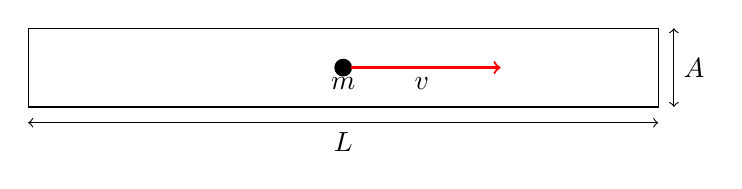
\begin{tikzpicture}[scale=4]
    \draw[draw=black] (0,0) rectangle(2,0.25);
    \filldraw (1,0.125) circle (0.75pt);
    \draw[red, ->, thick] (1.025,0.125) -- (1.5,0.125);
    \node[below] at (1,0.125) {$m$};
    \node[below] at (1.25,0.125) {$v$};
    \draw[<->] (0,-0.05) -- (2,-0.05);
    \draw[<->] (2.05,0) -- (2.05,0.25);
    \node[below] at (1,-0.05) {$L$};
    \node[right] at (2.05,0.125) {$A$};
    \end{tikzpicture}
\end{center}

Pictured above is our scenario; we have a single molecule of gas of mass $m$ and speed $v$ moving back and forth in a tube of length $L$, as it bounces off the ends of the tube that have area $A$. We assume that the molecule collides elastically off the walls, and hence it goes back and forth with velocities $\vec{v}$ and $-\vec{v}$. From our knowledge of kinematics, we obtain that the time it takes for the particle to go back and forth once is:
\begin{align*}
    \Delta t = \frac{2L}{v}
\end{align*}
Now, we want to figure out the average pressure that this particle applies on the wall; to obtain this, we, we return to how we have defined pressure above:
\begin{align*}
    P_{av} = \frac{F_{av}}{A}
\end{align*}
$A$ is just a constant here, so we then just need to figure out $F_{av}$! For this, we think back to the kinematics unit and the definition of force as the time derivative of momentum\footnote{Of course you know by know that force and momentum are vector and not scalar quantities, but since our problem is one dimensional, we can just consider the scalar version of the equation here!}:
\begin{align*}
    F = \frac{dp}{dt} = \frac{d(mv)}{dt}
\end{align*}
Since we are just concerned with the average force, we can just consider the change in momentum $\Delta p$ of the particle from hitting one of the ends over one cycle over the time it takes for one cycle (which is just $\Delta t$, above!). We consider that when the molecule hits the end of the tube with speed $v$, it reflects back elastically and starts going in the other direction with the same speed $v$, so its change in velocity is therefore $-2\Delta v$, and therefore the change in momentum is:
\[ \Delta p_{molecule} = -2m\Delta v\]
And therefore the average force applied to the wall is:
\[ F_{av} = \frac{-\Delta p_{molecule}}{\Delta t} = \frac{2mv}{\frac{2L}{v}} = \frac{mv^2}{L} \]
Then, getting the average pressure (from the one molecule) is simple, using the definition of pressure:
\[P_{av} = \frac{\frac{mv^2}{L}}{A} = \frac{mv^2}{V} \]
Where I have used the fact that the volume of the tube is given by $V = AL$. Now, in a real gas, we obviously don't just have one molecule, but a bunch of different molecules, all with different speeds! If we want the total pressure from a whole bunch of (say, $N$) molecules, we can just add up the average pressure of $N$ molecules:
\[P_{total} = \sum_{i=1}^N \frac{mv_i^2}{V}\]
As a reminder, the greek sigma $\Sigma$ above is telling us to take the "sum of N" things (in this case, molecules). It's clear that the volume can be taken out of the summation (because the volume of the tube is the same no matter which molecule we look at), and if we further assume that all of the masses of the molecules are the same (which is perfectly reasonable if we have a gas made of one element), then we obtain:
\[P_{total} = \frac{m}{V} \sum_{i=1}^N v_i^2 \]
Now I'm going to do a bit of a hack; I'm going to multiply this expression by $1 = \frac{N}{N}$:
\[P_{total} = N\frac{m}{V} \left(\frac{1}{N}\sum_{i=1}^N v_i^2 \right)\]
You might recognize from your physics labs that the quantity in brackets is just the \textit{average} of the squared velocities of all the molecules\footnote{To be clear, this is not the square of the averages!}; let us denote this by $v^2_{av}$. Now, let us multiply both sides by the volume $V$ of the box:
\[PV = Nmv^2_{av} \]
Now, if we multiply both sides by a half, we get something that looks familiar on the right hand side:
\[\frac{1}{2}PV = N\frac{1}{2}mv^2_{av} \]
You can see that we have exactly the average kinetic energy of our molecules (times the number of molecules in our system)! Now, at the beginning I said we were considering a one-dimensional system; but the direction we could have been talking about could have been the x direction, the y direction, or the z direction, and we would have got the same result! Therefore, we have that:
\[N\frac{1}{2}mv^2_{xav} = N\frac{1}{2}mv^2_{yav} = N\frac{1}{2}mv^2_{zav} = \frac{1}{2}PV \]
Therefore, for an ideal gas in three dimensions, all we have to do is add the three terms (the three kinetic energy contributions from each of the directions) together:
\begin{equation}
    \label{eqn:(2)}
    \frac{3}{2}PV = N\epsilon_{kavg}
\end{equation}
Where $\epsilon_{kavg}$ is the average kinetic energy of the molecules in three dimensions, defined as:
\begin{equation}
    \epsilon_{kavg} = \frac{1}{2}mv^2_{xav} + \frac{1}{2}mv^2_{yav} + \frac{1}{2}mv^2_{zav} = \frac{1}{2}m\vec{v}_{av} \cdot \vec{v}_{av}
\end{equation}
Now at this point, you might be holding your head in your hands because I spent three pages on a derivation\footnote{I sincerely apologize for your suffering.} and it seems like we're no closer to defining temperature than when we started. However, in the next section we will introduce the ideal gas law, and combining that with equation \ref{eqn:(2)} we just derived, we will see that we obtain exactly what we want to find. 
\subsection{The Ideal Gas Law and Definining Temperature}
Possibly the most important equation you'll encounter in thermodynamics is the ideal gas law. It states that
\begin{equation}
    \label{eqn:(4)}
    PV=Nk_{b}T
\end{equation}
where $P$ is the pressure of the gas (in Pascals), $V$ the volume (in $m^3$), $N$ the number of molecules of gas, $T$ the temperature (in \textbf{Kelvin})\footnote{Just as a refresher, x Kelvin = x-273 Celsius, and 0 Kelvin is absolute zero.}, and $k_b$ is Boltzmann's constant ($1.381 \times 10^{-23} \textrm{ m}^2 \textrm{ kg} \textrm{ s}^{-2} \textrm{ K}^{-1}$). We can consider this relationship as this as an empirical result; essentially, it is the combination of three simple gas laws that were determined experimentally. First, we had Boyle's Law, which tells us that for fixed temperature $T$ and amount of gas $N$, the pressure $P$ is inversely proportional to the volume $V$:
\begin{equation}
    P \propto \frac{1}{V}
\end{equation}
We then have Charles' Law, which tells us that for fixed pressure $P$ and amount of gas $N$, the volume $V$ is directly proportional to the temperature $T$:
\begin{equation}
    V \propto T
\end{equation}
Finally, we have Avogadro's Law, which tells us that for constant temperature $T$ and constant pressure $P$, The volume of gas $V$ is directly proportional to the amount $N$:
\begin{equation}
    V \propto N
\end{equation}
I will leave it to you to show that combining these three leads to the ideal gas law as we have stated it!\footnote{You can fairly easily show that this version of the gas law is equivalent to $PV=nRT$, the version you might be more familiar with; see the questions section!} \\
\noindent
Now, with everything we need in place, let's finally define temperature microscopically. Substituting equation \ref{eqn:(2)} from the previous section:
\begin{align*}
    \frac{3}{2}PV=N\epsilon_{kavg}
\end{align*}
And substituting in the ideal gas law, we get:
\begin{align*}
    \frac{3}{2}Nk_bT = N\epsilon_{kavg}
\end{align*}
Cancelling the $N$s and rearranging for the temperature $T$, we obtain:
\begin{equation}
    \label{eqn:(8)}
    T = \frac{2}{3k_b}\epsilon_{kavg}
\end{equation}
which seems like a good definition of temperature! What it essentially tells us is that the faster particles are moving in a gas on average, the hotter it is (although heavy particles can make up the difference, as mass also plays into kinetic energy).\\
\noindent
The final thing I should definitely mention is the long list of assumptions that equations \ref{eqn:(2)} and \ref{eqn:(4)} make. They are, in no particular order:
\begin{enumerate}
    \item A gas is made up of point-like particles of identical mass.
    \item The particles in a gas only interact via collisions.
    \item All collisions of particles in a gas are elastic.
\end{enumerate}
The above three conditions are what it means for a gas to be ideal. For those of you who followed along with the derivation of equation \ref{eqn:(2)}, you might recognize why these assumptions were necessary to make. \\
You might be tempted to ask; if equations \ref{eqn:(2)} and \ref{eqn:(4)} only hold for ideal gases, then does our new definition of temperature only hold for ideal gases as well? Actually, no! Even though the derivation we did for it used formulas that only applies to ideal gases, it turns out that the definition holds for \textbf{all} gases.
\subsection{Degrees of Freedom}
So there was something I neglected to explicitly tell you in the previous section\footnote{Hahahaha I'm so evil.}. Not all gases are ideal. In fact, most gases aren't ideal\footnote{Although most are almost ideal.}. Now's when I explain why this is. And to do that, I need to explain degrees of freedom.
\subsubsection{What are Degrees of Freedom?}
What a degree of freedom is can depend on the subject. For the purposes of thermodynamics, it's a way in which a particle can store energy. For example, the point-like particles that I talked about in ideal gas law can store energy in their motion along each directional axis. This gives them three degrees of freedom. That being said, there's a bunch of ways particles can store energy. They can vibrate, rotate, and have potential energy. The more of these a particle can do, the more degrees of freedom it has. However, not all degrees of freedom survive, because of reasons arising from quantum mechanics,\footnote{As you will learn next term, in quantum mechanics, energy is discretized (i.e. not continuous). If the amount of energy that could be stored in a potential degree of freedom is too small to get to the next discrete energy level, it'll be "frozen out". When that occurs, no energy can be stored in that way at all.} but essentially, each degree of freedom must store a minimum amount of energy to exist at all. 
\subsubsection{The Equipartition Theorem}
The equipartition theorem states that:
\begin{center}
    At thermal equilibrium, the thermal energy of a system is equally divided amongst all available degrees of freedom.
\end{center}
The equipartition theorem tells us that a a single quadratic degree of freedom \footnote{A quadratic degree of freedom is simply one where the energy goes by the square of some property; for example, the kinetic energy in the x direction is $E_{x} = \frac{1}{2}mv_x^2$, which is quadratic in the $v_x$ term.}, and therefore that one dimension of kinetic energy, has a magnitude of:
\begin{equation*}
    \epsilon_{k}=\frac{1}{2}{k_{b}}T.
\end{equation*}
 We also know that the total internal energy of the system is simply the sum of the energy of each particle. So
\begin{gather}
    E_{th}=\frac{\chi}{2}N{k_{b}}T \\
    E_{av}=\frac{\chi}{2}{k_{b}}T
\end{gather}
Here, $N$ represents the number of particles in the system, and $k_b$ is the Boltzmann constant, a fundamental constant of nature with a precisely defined value. $\chi$ is the number of degrees of freedom in a molecule, which happens to be $3$ for monotomic gases (corresponding to three translational degrees of freedom). A more comprehensive list is given in the section below. $T$ is temperature, in \textbf{Kelvin}. In questions 2 and 3 below, you will show that:
\begin{equation}
E_{th} = \frac{\chi}{2}nRT
\end{equation}
Where $n$ is the number of mols of gas, and $R$ is the gas constant ($R = 8.3145 \textrm{ J} \textrm{ mol}^{-1} \textrm{ K}^{-1}$). Now, we may define:
\[ c_v = \frac{\chi}{2}R \]
to be the specific heat capacity at a fixed volume. We now obtain the useful formula:
\begin{equation}
    E_{th} = nc_v T
\end{equation}
This formula is extremely useful for relating energy and temperature. Assuming that the amount and kind of gas you have doesn't change, this also allows us to look at the change in temperature and energy:
\begin{equation}
    \label{eqn:(13)}
    \Delta E_{th} = nc_v \Delta T
\end{equation}
The above formula will hold for any process where the amount of gas you have doesn't change, making it quite useful. It also has some immediately clear consequences. For one, it tells us that for a given amount of energy we give to a system, how much its temperature changes depends on two things; it depends on:
\begin{enumerate}
    \item The amount of stuff we have in the system, represented by the number of mols, $n$. This is fairly intuitive; the more stuff I have, the more energy I need to increase its temperature!
    \item The degrees of freedom of the molecules we are looking at. Imagine we were comparing two molecules, where one was simple molecule with few degrees of freedom (say, monotomic Helium), and a complex molecule with many degrees of freedom (say, a triatomic molecule), the former would have a lower heat capacity $c_v$ (check this from the definition!). Therefore, for a given amount of energy $\Delta E$ we give to a system, the system composed of molecules with fewer degrees of freedom will have a greater change in temperature (check this as well!). Physically, we might intuit this from the fact that molecules with a greater number of degrees of freedom have more degrees to which the energy can be distributed, and hence a smaller proportion of the energy goes into increasing the temperature. 
\end{enumerate}

Now, you may wonder why I have chosen to label $c_v$ the way I have (What do I mean by specific heat capacity at fixed volume?). This notation will soon become clear when we discuss the different thermodynamic processes. \\

Brief note before we move on; If you take the equipartition theorem to be a fundamental result\footnote{unfortunately, we will not be proving it here}, we obtain a derivation for our temperature definition in equation \ref{eqn:(8)} that works for any molecule (not just an ideal one). Any molecule in three dimensions would have three translational degrees of freedom, or three directions of kinetic energy. Therefore, the theorem would tell us that:
\[\epsilon_{kx}+\epsilon_{ky}+\epsilon_{kz} = \frac{1}{2}k_bT + \frac{1}{2}k_bT + \frac{1}{2}k_bT \]
So if we group the leftmost three terms into a general average kinetic energy term:
\[\epsilon_{kavg} = \frac{3}{2}k_bT \]
And rearranging for temperature:
\[T = \frac{2}{3k_b}\epsilon_{kavg} \]
So we have recovered our definition! In fact, you could combine this temperature definition with equation \ref{eqn:(2)} which we derived from first principles:
\[ \frac{3}{2} P V=N \epsilon_{kavg} \]
And actually derive the ideal gas law from scratch (without having to rely on it as an experimental result)!

\subsubsection{Degrees of Freedom of Different Molecule Types}
I've said that monoatomic, neutral gases have only three degrees of freedom. But as any good chemist knows\footnote{Don't confirm this with Chris or John} most elements don't like to be alone. So most gases aren't monoatomic. For example nitrogen gas, the most abundant gas in the atmosphere, is annoyingly diatomic. The ideal gas law doesn't apply to it (though, for reasonably low pressures\footnote{i.e. The range of pressures we would consider in Science One problems}, its behavior does not deviate far from an ideal gas, and we can apply the ideal gas law to it and be approximately correct. But the equation for energy does, if we could just figure out how many degrees of freedom it had, and the same is true for any gas. Anyways I'll stop prattling on now and tell you how many degrees of freedom these gases have (they're all kinetic degrees of freedom). \\
\newline
\begin{center}
\begin{tabular}{|c|c|c|}
    \hline
    Gas Type & \# of Deg of Freedom & Types of Deg of Freedom \\
    \hline
    Monoatomic & 3 & 3 translational \\
    \hline
    Diatomic & 5 & 3 translational, 2 rotational \\
    \hline
    Triatomic & 6 & 3 translational, 3 rotational \\
    \hline
\end{tabular}
\end{center}
\begin{figure}[h!]
    \centering
    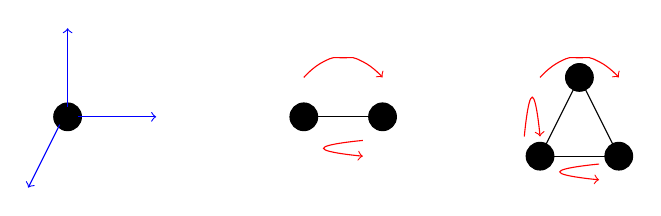
\begin{tikzpicture}
    \filldraw[fill=black, draw=black] (0,0) circle (5pt);
    \draw[->, blue] (0.13,0) -- (1.125,0);
    \draw[->, blue] (0,0.13) -- (0,1.125);
    \draw[->, blue] (-0.1,-0.1) -- (-0.5,-0.9);
    %\node[below] at (1,0) {$y$};
    %\node[left] at (0,1) {$z$};
    %\node[left] at (-0.5,-0.85) {$x$};
    
    \filldraw[fill=black, draw=black] (3,0) circle (5pt);
    \filldraw[fill=black, draw=black] (4,0) circle (5pt);
    \draw[black] (3,0) -- (4,0);
    \draw[->, red] plot [smooth, tension=1] coordinates {(3,0.5) (3.25,0.7) (3.5,0.75) (3.75,0.7) (4,0.5)};
    \draw[->, red] plot [smooth, tension=1] coordinates {(3.75,-0.3) (3.25,-0.4) (3.75,-0.5)};
    
    \filldraw[fill=black, draw=black] (6,-0.5) circle (5pt);
    \filldraw[fill=black, draw=black] (7,-0.5) circle (5pt);
    \filldraw[fill=black, draw=black] (6.5,0.5) circle (5pt);
    \draw[black] (6,-0.5) -- (7,-0.5);
    \draw[black] (6,-0.5) -- (6.5,0.5);
    \draw[black] (7,-0.5) -- (6.5,0.5);
    \draw[->, red] plot [smooth, tension=1] coordinates {(6,0.5) (6.25,0.7) (6.5,0.75) (6.75,0.7) (7,0.5)};
    \draw[->, red] plot [smooth, tension=1] coordinates {(6.75,-0.6) (6.25,-0.7) (6.75,-0.8)};
    \draw[->, red] plot [smooth, tension=1] coordinates {(5.8,-0.25) (5.9,0.25) (6,-0.25)};

    \end{tikzpicture}
    \caption{Visualization of the degrees of freedom of monoatomic, diatomic, and triatomic molecules. Monoatomic molecules only have three translational degrees of freedom, diatomic molecules have three translational plus two rotational degrees (it cannot rotate along the rotation axis parallel to its length), and the triatomic molecules have three translational and rotational degrees of freedom each.}
\end{figure}

\noindent
Liquids and solids have their own characteristic number of degrees of freedom too, I just didn't write them here. James/Chris might cover this in lecture however, so just because I didn't write it doesn't mean you don't need to know it\footnote{Really attach this disclaimer to the whole document}!
\newpage
\subsubsection{(Optional) Why Can't Monoatomic Molecules Rotate?}
After looking at that chart of degrees of freedom, you might be wondering: "Wait; why don't monoatomic gases have rotational degrees of freedom? What's stopping it from rotating?" The answer lies in the fact that the radius of atoms is extremely small; these leads to the atoms having a very small moment of inertia (you may recall that the moment of inertia of a sphere is $I = \frac{2}{5}MR^2$ where $M$ is the mass and $R$ the radius; if $R$ is small, then $R^2$ and therefore $I$ are extremely small). This has the consequence of the quantum energy levels of the rotational kinetic energy being extremely far apart. Hence these rotations are negligeble (i.e. not thermodynamically accessible) because they require a lot of energy to become excited; therefore, we do not consider the rotations as a degree of freedom\footnote{Since it's hard to get an intuition for why this is true, we can also consider a simpler (although oversimplified) explanation; if we approximate atoms as point particles of zero radius, then it becomes clear that they cannot rotate, and therefore the rotations cannot constitute a degree of freedom!}. You might be able to see why this argument generalizes to the diatomic molecule, as well (where you might have been wondering why it can't rotate along its length); the moment of inertia about the rotation axis along the length of the molecule is very small compared to the other two rotation axes; hence, rotations about that axis are not excited. 



\subsection{Practice Problems}
\begin{enumerate}
    \item Do particles in an ideal gas undergo inelastic or elastic collisions, and why? 
    \item \begin{enumerate}
        \item Using the relation $k_{b}N_A=R$ (where $R$ is the gas constant and $N_A$ is Avogadro's number, where $N_A = 6.02 \times 10^{23}$ is the number of molecules in a mole), show that $PV={k_{b}}NT$ is equivalent to $PV=nRT$.
        \item Using the relation from the previous part, along with $E_{th} = \frac{\chi}{2}Nk_bT$, show that $E_{th}=\frac{\chi}{2}nRT$.
        \item Express $E_{th}$ in terms of $\chi$, $P$ and $V$.
    \end{enumerate}
    \item If two systems have the same thermal energy, are they at the same temperature? Why?
    \item Imagine Raja is sitting perfectly still in the Science One Box\textsuperscript{TM}, a space specially designed for quiet study. To ensure complete silence, the space inside of the box is kept as a vacuum (don't worry there's a breathing tube). Is this box in equilibrium with its surroundings?
    \item Consider a very normal box\textsuperscript{TM} of very normal ideal gas\textsuperscript{TM}. What would happen to the gas if...
    \begin{enumerate}
        \item The volume of the box decreased?
        \item The volume of the box increased?
        \item The box sprang a leak?
    \end{enumerate}
    \item Imagine a box of particles that are the mass of IKB, which by some miracle don't collapse into black holes and are in fact completely stable. What would happen to the temperature of the gas if you increased the volume of the box, and why (Hint: Think about the gravitational potential energy, and not the ideal gas law)?
    \item Now, imagine a box filled with a gas composed entirely of electrons. When the volume of the box is decreased, what happens to the temperature of the gas, and why (Hint: This time, think about the electric potential energy)?
    \item Suppose you had two boxes of identical volume, with the particles in each travelling at the same average speed. How would the pressure and temperature of the boxes compare if
    \begin{enumerate}
        \item One box had more particles than the other?
        \item One box had heavier particles than the other?
    \end{enumerate}
    \item How much more energy would I have to supply to a triatomic molecule compared to a monoatomic molecule to get them to be the same temperature? Why?
    \item How many degrees of freedom would a monatomic molecule have in 10 dimensional space\footnote{Hurray for string theory!}? If I were to give the same amount of energy to 3 dimensional and 10 dimensional helium, which would have a greater change in temperature?


\end{enumerate}
\newpage
\section{\texorpdfstring{The 1\textsuperscript{st} Law of Thermodynamics}{The 1st Law of Thermodynamics}}
This section is on the first law of thermodynamics and its many, many applications. It's not the most conceptually difficult of the laws, but it will probably be the one that shows up the most on your midterm.
\subsection{Mechanical and Non-Mechanical Energy}
The 1\textsuperscript{st} law is all about the mechanical and non-mechanical transfer of energy, so its important that we understand the difference between the two. A mechanical transfer of energy is work. A non-mechanical transfer of energy is any transfer of energy that does no work. For example, say you put a pot on a hot stove-top. The pot will heat up, so it's obviously gaining energy, but there's no motion and therefore no work being done. Any non-mechanical transfers of energy like this are called heat\footnote{You can't say something "has heat" in the same way you can't say something "has work"!}.
\subsection{\texorpdfstring{The 1\textsuperscript{st} Law of Thermodynamics}{The 1st Law of Thermodynamics}}
Let $\Delta E$ be the change in energy of a system, $Q$ be the heat that flows in/out the system, and W the work done on the system. The first law of thermodynamics simply states that the total change in energy of a system is equal to the sum of its mechanical and non-mechanical transfers of energy, or
\begin{equation}
    \Delta E=Q+W
\end{equation}
Be careful with the signs when using this equation! For example, had I defined $W$ as the amount of work done \textit{by} the system, this equation would instead be
\begin{equation*}
    \Delta E=Q-W
\end{equation*}
It is worth noting here that while $W$ and $Q$ are both \textbf{functions of path}; how much work I do or a system does, or how much heat flows in/out of a system depends on how a process happens. However, internal energy is a \textbf{function of state}; it depends only on the current state of the system, but not how the system got there. The moral is that while how a system might gain or lose energy is a function of the path, the internal energy itself is a function of the state of the system only.
\subsection{Defining Work on a Gas}
As you may remember from the previous unit, work is generally defined as
\begin{equation}
    W = \int_{x_1}^{x_2} Fdx
\end{equation}
However, in thermodynamics we don't have position or force as variables to work with. Instead, we have pressure and volume. So, we need to find a way to define force and position in terms of pressure and volume. Starting with force, I can say that $F = PA$, so substituting that into the equation we get
\begin{equation*}
    W = \int_{x_1}^{x_2} PAdx
\end{equation*}
The product of area and distance is volume (Think of a cube. What's the area of on of the cube's faces times the length of its side?). So, since dx is a tiny displacement, which ultimately is a length, Adx is a tiny change in volume! Therefore:
\begin{equation*}
    W = \int_{V_1}^{V_2} PdV
\end{equation*}
However, there's one more issue with this. The way I've defined work so far was based on the definition of the amount of work done \textbf{by} a system on another system. We want the amount of work done \textbf{on} the system. Due to conservation of energy, I can just throw a negative sign in front to get
\begin{equation}
    W = -\int_{V_1}^{V_2} PdV
\end{equation}
This is the proper definition of the work done on a gas. One thing to be careful of here; It looks like the pressure $P$ is just a constant I can take out of the integral. This is only the case if the pressure is \textit{actually a constant over the entire process}. Otherwise, the pressure really is a function of volume, and so we keep it inside the integral; to be extra clear that the pressure is changing as a function of volume, we should write the equation as:
\begin{equation}
    \label{eqn:(16)}
    W = -\int_{V_1}^{V_2} P(V)dV
\end{equation}
The below diagram illustrates gas in a box with a piston, and shows the work done by the gas (because it's easier to draw):
\begin{center}
    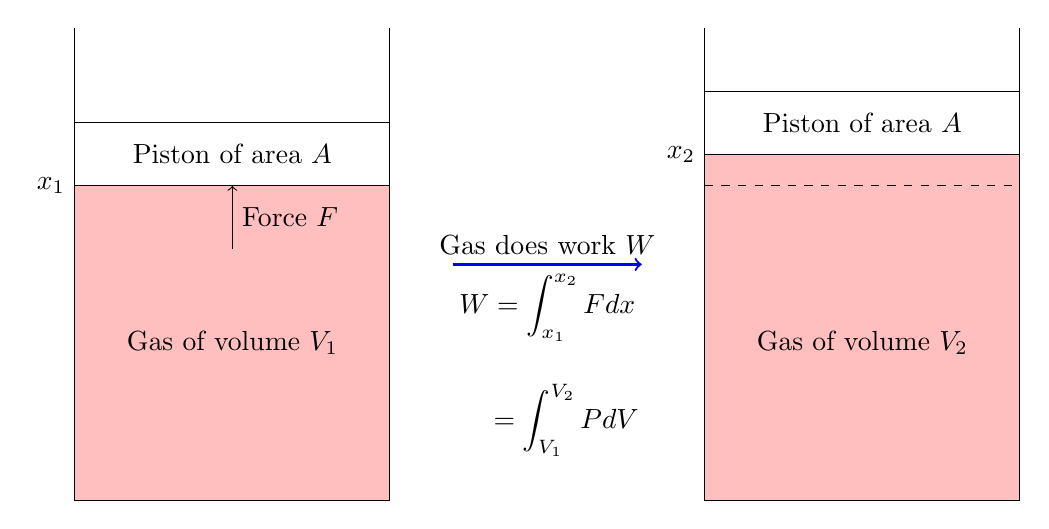
\begin{tikzpicture}[scale=4]
    \filldraw[fill=pink, draw = black] (0,0) rectangle (1,1);
    \draw[black] (0,1) rectangle (1,1.2);
    \draw (0,1.2) -- (0,1.5);
    \draw (1,1.2) -- (1,1.5);
    \draw[->] (0.5,0.8) -- (0.5,1);
    \node[right] at (0.5,0.9) {Force $F$};
    \node[left] at (0,1) {$x_1$};
    \draw (0.5,0.5) node {Gas of volume $V_1$};
    \draw (0.5, 1.1) node {Piston of area $A$};
    \draw[->, blue, thick] (1.2,0.75) -- (1.8, 0.75);
    \node[above] at (1.5,0.75) {Gas does work $W$};
    \node[below] at (1.5,0.75) {$\displaystyle W = \int_{x_1}^{x_2} Fdx$};
    \node[below] at (1.5,0.4) {$\displaystyle \phantom{W }=  \int_{V_1}^{V_2} PdV$};
    \filldraw[fill=pink, draw = black] (2,0) rectangle (3,1.1);
    \draw[black] (2,1.1) rectangle (3,1.3);
    \draw[dashed] (2,1) -- (3,1);
    \draw (2,1.2) -- (2,1.5);
    \draw (3,1.2) -- (3,1.5);
    \node[left] at (2,1.1) {$x_2$};
    \draw (2.5,0.5) node {Gas of volume $V_2$};
    \draw (2.5, 1.2) node {Piston of area $A$};
    \end{tikzpicture}
\end{center}

\subsection{PV Diagrams}
Like all things in physics, physicists really enjoy graphing thermodynamic processes. Their particular favorite is the PV graph, putting pressure on the y-axis and volume on the x-axis; from the ideal gas law, you may see why this is a natural choice of axes. Shown below is a PV graph of a thermodynamic process that takes the gas from starting temperature $T_1$ (at pressure $P_1$ and volume $V_1$) to temperature $T_2$ (at pressure $P_2$ and volume $V_2$). Of course, there's nothing stopping us from assigning numbers to $P,T,V$, as well, if the situation calls for it. The process pictured below is an expansion of the gas, but we could also very well draw the arrow the other way and depict a compression of the gas. 
\begin{center}
\begin{tikzpicture}
 \draw[stealth-stealth] (0,5) node[below left]{$P$} |- (5,0) node[below left]{$V$};
 \draw[thick,->] (1,4) -- (2.5,2.5);
\draw[thick] (2.5,2.5) -- (4,1);
\draw[dashed] (4,0) -- (4,1);
\draw[dashed] (1,0) -- (1,4);
\draw[dashed] (4,1) -- (0,1);
\draw[dashed] (1,4) -- (0,4);
\filldraw (1,4) circle (2pt);
\filldraw (4,1) circle (2pt);
\node[below] at (1,0) {$V_1$};
\node[below] at (4,0) {$V_2$};
\node[left] at (0,1) {$P_2$};
\node[left] at (0,4) {$P_1$};
\node[right] at (1,4) {$T_1$};
\node[right] at (4,1) {$T_2$};
 \end{tikzpicture}
 \end{center}
 To get a feel for these kinds of graphs, I would suggest trying to make some. Write down an initial state and final state for your gas with one or two quantities remaining constant, and try to figure out what the graph between those two steps would look like. For example, if I had
\begin{itemize}
    \item Initial State: P = 10kPa, V = 1m$^3$, N = 10molecules, T = 300K
    \item Final State: P = 5kPa, V = 2$m^3$, N = 10molecules, T = 300K
\end{itemize}
What would the graph between the two states look like if temperature and number of molecules were held constant the entire time? (Hint: You might be first inclined to think it looks like a diagonal line like the diagram above, but this isn't quite correct; think about why the condition of temperature being held constant for the entire time might not hold in this case). The answer will be revealed very shortly, when we discuss the PV diagrams of the 4 basic thermodynamic processes! \\
Before we go there though, there is one very useful connection between PV diagrams and work that I would like to point out. In the previous section, we defined the work done on the gas as:
\[ W = -\int_{V_1}^{V_2} P(V)dV \]
And looking at the PV diagram, it now becomes clear that this is nothing more than the (negative) area under the PV curve! As an example, let's figure out the work done on the gas in the process shown above. All we have to do is calculate the area underneath the curve. For convenience, let us split it into two parts of the triangle and the rectangle. For the triangle, we have area $\frac{1}{2}*\left(P_1-P_2\right)*\left(V_2-V_1\right)$, and for the rectangle, we have area $P_2*\left(V_2-V_1\right)$. Therefore, the total area under the graph is:
\[ \text{Area } = \frac{1}{2}*\left(P_1-P_2\right)*\left(V_2-V_1\right) + P_2*\left(V_2-V_1\right) = \frac{1}{2}\left[\left(P_1+P_2\right)\left(V_2-V_1\right) \right]\]
This area is in fact the work done \textbf{by} the gas, and the work done on the gas is just its negative:
\[W_{on} = \frac{1}{2}\left[\left(P_1+P_2\right)\left(V_1-V_2\right) \right]\]
When using this area argument, do be careful of which direction the curve is going; for example, if the process was a compression of the gas rather than an expansion, we would have to introduce a negative sign as things would be going in the opposite direction. 

\subsection{Thermodynamic Processes}
This subsection is devoted to all the different types of thermodynamic processes that we talk about in this course. Note that in all of these processes, we have that some quantity is held constant/is zero (e.g. volume, pressure, temperature, or no heat flow). Nearly all processes you will see in this course and in your exams will be one of these four types, but don't assume it will be unless you can justify it. Also note that there are quite a few derivations in this section (e.g. deriving the work done in an isothermal process). This is mainly to aid your understanding, and for exams, you can just use the final results to calculate whatever is relevant without worrying about the derivation. 
\subsubsection{Isochoric Processes}
Isochoric processes are heating/cooling processes where the volume of the gas does not change ($\Delta V =0$). For example, consider a situation where I have a gas in a closed box with rigid walls. Now, imagine I heat up the gas by holding a lighted candle underneath it. It is clear that the gas does not change in volume, as the walls are rigid (there is nothing it can expand out to, or for it to be compressed by), but we are changing the energy of the gas. Let's look at the properties of this process a little more closely.\\

Firstly, what is the work that's done in this process? This one's fairly simple; We can return to the definition \[ W = -\int_{V_1}^{V_2} P(V)dV \] and we realize that as there is no change in volume, $V_1 = V_2$ and therefore: \[ W = -\int_{V_1}^{V_1} P(V)dV = 0 \]
\begin{equation}
    W=0
\end{equation}
and the work done is zero! Combining this with the first law of thermodynamics, we have that: \[\Delta E = Q + W = Q \]
where we see that the change in energy is just the heat that flows in/out of the system, as we might have expected. Finally, as we know that $\Delta E = Q$, we also obtain the heat as a function of the change in temperature and amount (and degrees of freedom!) of the gas:
\begin{equation} 
Q = nc_v\Delta T
\end{equation}
Our earlier question about why we have called $c_v$ as we have is now answered! We can see from here that $c_v = \frac{\chi}{2}R$ is equivalent to the heat capacity of a material, where we have fixed the volume. \\Finally, we may ask what might this process look like on a PV-diagram? Let's return to the candle example. As we heat the gas up, the volume of the gas remains unchanged, so the process should be a graph of a line with constant $V$. Conversely, as the gas goes from a lower temperature $T_1$ to a higher temperature $T_2$, we would expect the pressure to increase. Hence, on a PV diagram, we would expect a straight vertical line:
\begin{center}
    \begin{tikzpicture}
 \draw[stealth-stealth] (0,5) node[below left]{$P$} |- (5,0) node[below left]{$V$};
\draw[thick,->] (2.5,1) -- (2.5,2.5);
\draw[thick] (2.5,2.5) -- (2.5,4);
\draw[dashed] (2.5,1) -- (2.5,0);
\draw[dashed] (2.5,1) -- (0,1);
\draw[dashed] (2.5,4) -- (0,4);
\filldraw (2.5,1) circle (2pt);
\filldraw (2.5,4) circle (2pt);
\node[below] at (2.5,0) {$V_1$};
\node[left] at (0,1) {$P_1$};
\node[left] at (0,4) {$P_2$};
\node[right] at (2.5,1) {$T_1$};
\node[right] at (2.5,4) {$T_2$};
\end{tikzpicture}
\end{center}
It's also very easy to see just from this graph that isochoric processes have zero work; The area under a curve on a PV-diagram yields the work done in that process, but a straight vertical line obviously has no area. 
\subsubsection{Isobaric Processes}
Isobaric processes are compression/expansion processes in which the pressure of the gas does not change ($\Delta P = 0$). For example, consider a box of gas where the top face is a piston. If I heat up the gas with a candle, then the piston gets pushed up by the warming, expanding gas, while the pressure of the gas stays constant.  \\

First, let us determine the work done on the gas in this process:
\[W = -\int_{V_1}^{V_2} P(V)dV \]
As $P$ is a constant, we can just take it outside the integral, and this becomes a very straightforward integration:
\[W = -P\int_{V_1}^{V_2} dV = -P \cdot \left. V \right|_{V_1}^{V_2} = -P(V_2-V_1) = -P\Delta V\]
\begin{equation}
    W = -P\Delta V
\end{equation}
Which is exactly as we would have expected. \\

Now that we know what the work done in an isobaric process is, we can consider the heat flow. We return to the first law of thermodynamics:
\[ \Delta E = W + Q \]
We recall that the following formula (from section 1) always holds true for change in energy:
\[ \Delta E = nc_v\Delta T = n \frac{\chi}{2}R\Delta T \]
We substitute the formulas for work and change in energy we have obtained:
\[ n \frac{\chi}{2}R\Delta T  = -P\Delta V + Q \]
Now, we use the ideal gas law to recognize that:
\[ P\Delta V = nR \Delta T \]
Making this subtitution, we have:
\[ n \frac{\chi}{2}R\Delta T = -nR \Delta T + Q \]
Combining the like terms, we have:
\[ Q = nR\left(\frac{\chi}{2}+1\right)\Delta T \]
Now, let us define the heat capacity at constant pressure:
\begin{equation}
c_p = \left( \frac{\chi}{2}+1 \right)R = c_v+R
\end{equation}
Which gives us the formula for the heat in an isobaric process:
\begin{equation}
    Q = nc_p \Delta T
\end{equation}
You may very well recognize this formula from high school physics or chemistry! Something of interest to point out here; we notive that $c_p>c_v$, or that the heat capacity at constant pressure is higher than the heat capacity at constant volume. This tells us that when something is allowed to expand as it is heated (retaining constant pressure), it requires more energy to increase its temperature than if it is kept at a fixed volume.
\\
Finally, let's consider what an isobaric process looks like on a PV diagram. As you might suspect, since we fix $P$ and let $V$ vary throughout the whole process, we yet again get a straight line, except this time a horizontal one. Pictured below is an isothermal expansion:

\begin{center}
    \begin{tikzpicture}
 \draw[stealth-stealth] (0,5) node[below left]{$P$} |- (5,0) node[below left]{$V$};
\draw[thick,->] (1,2.5) -- (2.5,2.5);
\draw[thick] (2.5,2.5) -- (4,2.5);
\draw[dashed] (0,2.5) -- (1,2.5);
\draw[dashed] (1,0) -- (1,2.5);
\draw[dashed] (4,0) -- (4,2.5);
\filldraw (1,2.5) circle (2pt);
\filldraw (4,2.5) circle (2pt);
\node[below] at (4,0) {$V_2$};
\node[below] at (1,0) {$V_1$};
\node[left] at (0,2.5) {$P_1$};
\node[above] at (1,2.5) {$T_1$};
\node[above] at (4,2.5) {$T_2$};
\end{tikzpicture}
\end{center}
Again, for visual confirmation of our result for work during an isobaric process, we can see that the (negative) area under the curve is $-P_1\Delta V$, by inspection. 
\subsubsection{Isothermal Processes}
Isothermal processes are compression/expansion processes in which the temperature of the gas remains constant ($\Delta T = 0$). These processes occur very slowly. As an example, we consider a scenario where I have some gas in a cylinder (closed off at the top by a piston), where I push down on the piston very very slowly. Doing so, the gas inside the piston remains at thermal equilibrium with its surroundings. Hence, I as I do work on the gas, an equal amount of energy leaves the gas in the form of heat, and the gas inside the piston stays at the same temperature. \\
\noindent
One immediate consequence that we obtain from $\Delta E = nc_v\Delta T$ is that:
\begin{equation}
    \Delta E = 0
\end{equation}
And by the first law of thermodynamics, we have that:
\begin{equation}
    W = -Q
\end{equation}
What exactly is the amount of work done in an isothermal process? We once again return to the definition of work:
\[ W = -\int_{V_1}^{V_2}P(V)dV \]
We have to be very careful here though; in this situation, the pressure is not constant as we vary/integrate over the volume. So we have to be a bit clever, and think of a way in which we can express the pressure as a function of volume so we can carry out the integral. If your intution was "ideal gas law", then you'd be exactly right! Let us make the substition:
\[ P(V) = \frac{nRT}{V} \]
Which turns the integral into:
\[ W = -\int_{V_1}^{V_2}nRT\frac{dV}{V}\]
Throughout this process $T$ is held constant, and the amount of gas does not change, so we can take most of the terms out of the integral as a constant:
\[ W = -nRT\int_{V_1}^{V_2}\frac{dV}{V}\]
The remaining integral is straightforward:
\[ W = -nRT \left. \ln(V) \right|_{V_1}^{V_2} = -nRT\left(\ln(V_2)-\ln(V_1)\right) = nRT\left(\ln(V_1)-\ln(V_2)\right) \]
So applying some laws of logarithms, we hence obtain our expression for the work done on the gas in an isothermal process:
\begin{equation}
W = nRT\ln\left(\frac{V_1}{V_2}\right)
\end{equation}
As we found earlier, the heat flow during an isothermal process is simply the negative of this, so:
\begin{equation}
    Q = -nRT\ln\left(\frac{V_1}{V_2}\right) = nRT\ln\left(\frac{V_2}{V_1}\right)
\end{equation}
\noindent
Finally, we consider how isothermal curves show up on PV diagrams. From how the expression for the work looks (with the $\ln$ term), you may suspect that we might get a "curved" curve rather than a straight diagonal line, and you would be right. Pictured here is an isothermal expansion from initial state $P_1,V_1$ to final state $P_2,V_2$. The temperature stays constant at every point on the curve. 

\begin{center}
    \begin{tikzpicture}
    \begin{axis}[
        axis x line=bottom,
        axis y line=left,
        xmin=0, xmax=10,
        ymin=0, ymax=10,
%        % (made labels more common)
%        % (because of the "sketch" type of the plot these should not be needed)
%        xlabel={Volume $(\mathrm{m}^3)$},
%        ylabel={Pressure (Pa)},
        % (changed ticks + labels to normal ticks instead of extra ticks)
        xtick={3,6},
        xticklabels={$V_1$,$V_2$},
        ytick={1.5,6},
        yticklabels={$P_2$,$P_1$},  % <-- (changed order of entries)
    ]
        % fill the area below the curve
        % (draw it first, so it is below everything else)


        % draw the dashed lines
        % (using two different approaches)
        \addplot [dashed,domain=0:3,samples=2] {6};
        \addplot [dashed,domain=0:6,samples=2] {1.5};

        \draw [dashed,thin] (axis cs:6,1.5) -- (axis cs:6,0);
        \draw [dashed,thin] (axis cs:3,6)   -- (axis cs:3,0);

        % now draw the curve
        \draw [
            fleche={0.6:black},              % <-- added
        ] (axis cs:3,6) to [bend right=30]
            % store start and end coordinates
            coordinate [pos=1] (start)
            coordinate [pos=0] (end)
        (axis cs:6,1.5);

        % draw start and end point
        \fill [radius=2pt]
            (start) circle[]
            (end)   circle[];
    \end{axis}
        \node[below] at (6.5,0) {$V$};
        \node[left] at (0,5.5) {$P$};
        \node[right] at (2.2,3.4) {$T_1$};
        \node[right] at (4.25,0.9) {$T_1$};
\end{tikzpicture}
\end{center}

\subsubsection{Adiabatic Processes}
Adiabatic processes are compression/expansion processes in which the gas has no heat flow ($Q=0$). These processes tend to be either fast, or occur under insulated conditions; for example, consider the same gas cylinder with the piston we discussed in the isothermal section. If instead of pushing in the piston very slowly, we push down forcefully, the compression will occur so quickly that there wouldn't be time for heat to flow out of the gas. This would be an adiabatic compression. As another example, if we had a cylinder of gas surrounded with thermal insulation, then even if we were to compress the piston or let the gas expand, there would be no heat flow and again we would have an adiabatic process.Let's consider some mathematical consequences of adiabatic processes. As a consequence of zero heat flow, by the first law of thermodynamics we have that:
\begin{equation}
    \Delta E = W
\end{equation}
So then for an adiabatic process, we can get that:
\begin{equation}
    W = \frac{\chi}{2}N{k_b}\Delta T
\end{equation}
I'm also going to show the derivation for the other relation relevant to adiabatic processes. The derivation is beyond the scope of this course, so if you don't want to read it just skip to the final equations we obtain at the end end\footnote{My disappointment will be immeasurable and my day ruined if you do}. This derivation first takes the relation in (20) for an infinitesimal step, then runs some rearrangement before integrating:
\begin{align*}
    dE &= \delta W \\
    \frac{\chi}{2}N{k_b}dT &= -PdV
\end{align*}
Like in the isothermal case, we make a substitution with ideal gas law, namely
\begin{equation*}
    N{k_b}dT = d(PV)
\end{equation*}
I also use the approximation $d(PV) = VdP + PdV$\footnote{As for why, play around with $d(PV) = (P+dP)(V+dV) - PV$... or just consider the product rule.}. Making all of these substitutions gives
\begin{equation*}
    \frac{\chi}{2}(VdP + PdV) = -PdV
\end{equation*}
At this point you have all the parts necessary to rearrange this equation into
\begin{equation*}
    \frac{\chi}{2}\frac{dP}{P} = -\Big(\frac{\chi}{2} + 1\Big)\frac{dV}{V}
\end{equation*}
If you guessed that we integrate both sides of this equation, then you're right! This may seem a bit strange, since we're integrating the two sides of the equation against two different variables, but it is in fact perfectly legal. By integrating, we're taking a sum on both sides of all the infinitesimal steps from the initial to final state. Since both sides are using the same initial and final state, it makes sense that taking small steps between them should always yield the same result. Anyways, integrating this equation gives:
\begin{equation*}
    \int_{P_1}^{P_2} \frac{\chi}{2}\frac{dP}{P} = \int_{V_1}^{V_2} -\Big(\frac{\chi}{2} + 1\Big)\frac{dV}{V}
\end{equation*}
Again, we can factor out the constant terms to get:
\begin{equation*}
    \frac{\chi}{2}\int_{P_1}^{P_2} \frac{dP}{P} = -\Big(\frac{\chi}{2} + 1\Big)\int_{V_1}^{V_2} \frac{dV}{V}
\end{equation*}
At this point the integral on each side evaluates in the exact same way as when we integrated to get isothermal work done:
\begin{equation*}
    \frac{\chi}{2}\ln{\Big(\frac{P_2}{P_1}\Big)} = -\Big(\frac{\chi}{2} + 1\Big)\ln{\Big(\frac{V_2}{V_1}\Big)}
\end{equation*}
Multiplying both sides of this equation by $\frac{2}{\chi}$ yields:
\begin{equation*}
    \ln{\Big(\frac{P_2}{P_1}\Big)} = -\Big(\frac{\chi+2}{\chi}\Big)\ln{\Big(\frac{V_2}{V_1}\Big)}
\end{equation*}
We then take the natural exponent of both sides of the equation to get:
\begin{align*}
    e^{\ln{\big(\frac{P_2}{P_1}\big)}} &= e^{-\big(\frac{\chi+2}{\chi}\big)\ln{\big(\frac{V_2}{V_1}\big)}} \\
    \frac{P_2}{P_1} &= e^{\ln{\Big(\big(\frac{V_2}{V_1}\big)^{-\big(\frac{\chi+2}{\chi}\big)}\Big)}} \\
    \frac{P_2}{P_1} &= \Big(\frac{V_2}{V_1}\Big)^{-\big(\frac{\chi+2}{\chi}\big)}
\end{align*}
Raise both sides to the exponent -1, rearrange a bit, and you get:
\begin{equation}
    {P_1}{V_1}^{\frac{\chi+2}{\chi}} = {P_2}{V_2}^{\frac{\chi+2}{\chi}}
\end{equation}
Sometimes the quantity $\frac{\chi+2}{\chi}$ is called $\gamma$ as well. Note that this identity we have discovered can take some alternative forms (which can be useful for exams); for example, making the subtitution $P = \frac{nRT}{V}$, we get:
\[ \frac{nRT_1}{V_1}V_1^\gamma = \frac{nRT_2}{V_2}V_2^\gamma \]
And cancelling out $nR$ on both sides and grouping like terms, we obtain the formula:
\begin{equation}
    T_1V_1^{\gamma-1} = T_2V_2^{\gamma-1}
\end{equation}
Finally, we again consider what an adiabatic process looks like on a PV diagram; the visual answer is that it looks quite a bit like the isothermal curve, but is steeper/lies above it. You can see both curves pictured below for comparison. The adiabatic expansion is pictured in black, and the isothermal curve in dashed red:
\begin{center}
    \begin{tikzpicture}
    \begin{axis}[
        axis x line=bottom,
        axis y line=left,
        xmin=0, xmax=10,
        ymin=0, ymax=10,
%        % (made labels more common)
%        % (because of the "sketch" type of the plot these should not be needed)
%        xlabel={Volume $(\mathrm{m}^3)$},
%        ylabel={Pressure (Pa)},
        % (changed ticks + labels to normal ticks instead of extra ticks)
        xtick={3.75,6},
        xticklabels={$V_1$,$V_2$},
        ytick={1.5,6},
        yticklabels={$P_2$,$P_1$},  % <-- (changed order of entries)
    ]
        % fill the area below the curve
        % (draw it first, so it is below everything else)


        % draw the dashed lines
        % (using two different approaches)
        \addplot [dashed,domain=0:3.75,samples=2] {6};
        \addplot [dashed,domain=0:6,samples=2] {1.5};

        \draw [dashed,thin] (axis cs:6,1.5) -- (axis cs:6,0);
        \draw [dashed,thin] (axis cs:3.75,6)   -- (axis cs:3.75,0);

        % now draw the curve
        \draw [
            dotted,red             % <-- added
        ] (axis cs:3,6) to [bend right=30]
            % store start and end coordinates
            coordinate [pos=1] (start)
            coordinate [pos=0] (end)
        (axis cs:6,1.5);
        
        \draw [
            fleche={0.6:black}            % <-- added
        ] (axis cs:3.75,6) to [bend right=30]
            % store start and end coordinates
            coordinate [pos=1] (start)
            coordinate [pos=0] (end)
        (axis cs:6,1.5);
        
        
        % draw start and end point
        \fill [radius=2pt]
            (start) circle[]
            (end)   circle[];
        \node[right] at (axis cs:6,1.5) {$T_2$};
        \node[right] at (axis cs:3.75,6) {$T_1$};
    \end{axis}
        \node[below] at (6.5,0) {$V$};
        \node[left] at (0,5.5) {$P$};

\end{tikzpicture}
\end{center}
\subsection{Heat Engines \& The Carnot Cycle}
Perhaps one of the most useful applications of thermodynamics is the development of heat engines (and heat pumps, which are just their inverse). With everything we have just discussed, we have basically all the tools we need to discuss and understand how heat engines work\footnote{Unintentional pun}. We will start by introducing a very abstract model for a heat engine, and then try to cement our understanding with a more concrete example. \\

In essence, a heat engine is a medium (in the context of Science One, a purely gaseuous medium\footnote{Sorry steam engines... you'll have to wait until second year}) that you can supply energy to in the form of heat, and you will get back some energy in the form of useful work. The end goal of the heat engine is to do as much work for us as possible. Essentially, the process goes as follows:
\begin{enumerate}
    \item The heat engine starts in its original state.
    \item The heat engine accepts some heat $Q_H$ from an external hot bath of temperature $T_H$.
    \item The heat engine does work $W$ from the energy given to it in the form of heat.
    \item The heat engine throws away some "waste heat" $Q_C$ into a cold bath of temperature $T_C$.
    \item The heat engine returns to its original state, and the cycle begins again.
\end{enumerate}
This is demonstrated in a diagram below. Note that this is just a general outline, but really steps 2-4 can occur in a different order, multiple times, and sometimes concurrently. A diagram illustrates this below:
\begin{center}
    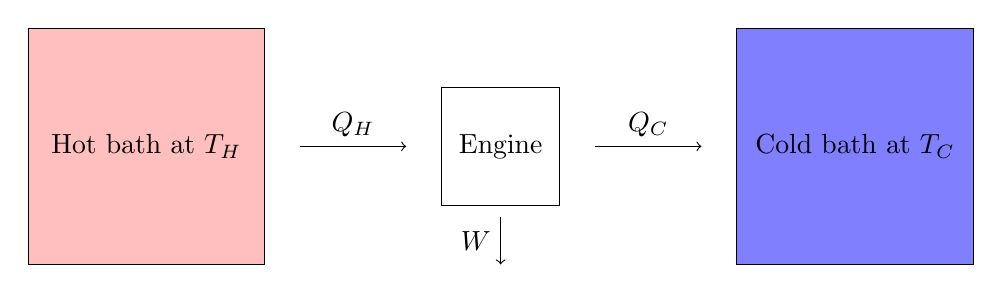
\begin{tikzpicture}[scale=3]
    \filldraw[fill=pink] (0,0) rectangle (1,1);
    \draw (1.75,0.25) rectangle (2.25,0.75);
    \filldraw[fill=blue!50] (3,0) rectangle (4,1);
    \draw[->] (1.15,0.5) -- (1.6,0.5);
    \draw[->] (2.4,0.5) -- (2.85,0.5);
    \draw[->] (2,0.2) -- (2,0);
    \node[above] at (1.375,0.5) {$Q_H$};
    \node[above] at (2.625,0.5) {$Q_C$};
    \node[left] at (2,0.1) {$W$};
    \draw (2,0.5) node {Engine};
    \draw (0.5,0.5) node {Hot bath at $T_H$};
    \draw (3.5,0.5) node {Cold bath at $T_C$};=
    \end{tikzpicture}
\end{center}
Of course, we could also flip the direction in which we do things to give the opposite result, which results in a heat pump! Instead of putting heat at a high temperature $T_H$ to get work $W$ out, I can instead supply the heat engine with heat $Q_C$ at a low temperature $T_C$ (which is very cheap) and then supply work to the heat engine to get heat $Q_H$ out at a high temperature.  \\
A measure of how good a heat engine is is given by its efficiency. Clearly, we want to be getting as much useful work $W$ out of the steam engine from the energy/heat $Q_H$ that we are putting into it! Then, a very natural measure of the efficiency becomes:
\begin{equation}
    \eta = \frac{W}{Q_H} = \frac{W_{net}}{Q_{in}}
\end{equation}
We can observe that this efficiency measure is a percentage; It can range from $0$ (where $W=0$ and we have a broken heat engine) to $1$ (where $W=Q_H$ and we have a perfect conversion of the energy we put in to the work we get out). However, we will soon see that a 100\% efficient heat engine is not realistic at all; this would require that no waste heat $Q_C$ is produced at all, which is realistically impossible. In fact, in a little while we will introduce a theoretical maximum for just how efficient a heat engine can be!
\subsubsection{Heat Engines on PV diagrams}
As you might have guessed from all the time we spent setting up how different thermodynamic processes look on PV diagrams, a great way for representing heat engines is to draw them as a closed, non-intersecting curve\footnote{The curve has to end where it began, else the heat engine won't be in the same place where it started after one cycle!} on a PV diagram! Let's illustrate this with an example. Pictured below is a representation of a simple heat engine. For simplicity, let's imagine that the gas medium is 1 mole of monoatomic gas (with 3 degrees of freedom). 

\begin{center}
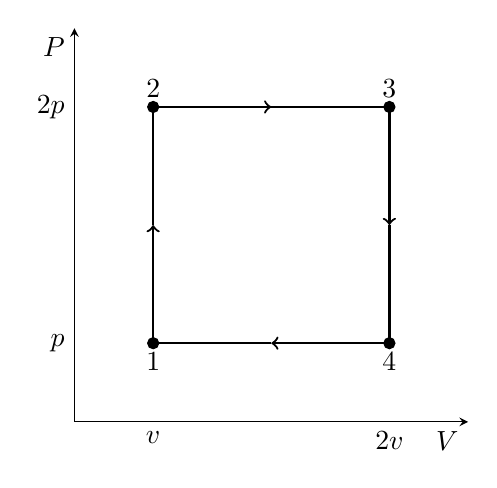
\begin{tikzpicture}
 \draw[stealth-stealth] (0,5) node[below left]{$P$} |- (5,0) node[below left]{$V$};
\filldraw (1,1) circle (2pt);
\filldraw (4,1) circle (2pt);
\filldraw (4,4) circle (2pt);
\filldraw (1,4) circle (2pt);

\draw[thick,->] (1,4) -- (2.5,4);
\draw[thick] (2.5,4) -- (4,4);
\draw[thick,->] (4,4) -- (4,2.5);
\draw[thick] (4,2.5) -- (4,1);
\draw[thick,->] (4,1) -- (2.5,1);
\draw[thick] (2.5,1) -- (1,1);
\draw[thick,->] (1,1) -- (1,2.5);
\draw[thick] (1,2.5) -- (1,4);

\node[above] at (1,4) {$2$};
\node[above] at (4,4) {$3$};
\node[below] at (4,1) {$4$};
\node[below] at (1,1) {$1$};

%\draw[dashed] (0,4) -- (1,4);
%\draw[dashed] (0,1) -- (1,1);
%\draw[dashed] (1,0) -- (1,1);
%\draw[dashed] (4,0) -- (4,1);

\node[below] at (4,0) {$2v$};
\node[below] at (1,0) {$v$};
\node[left] at (0,1) {$p$};
\node[left] at (0,4) {$2p$};
\end{tikzpicture}
\end{center}

What exactly can we get out of this graph? There's a lot of information packed into it, so to start, let's break it down into the individual steps of the heat engine. The gas in the engine starts at state $1$, at pressure $p$ and volume $v$. We heat the gas isochorically, giving it heat, until it reaches state $2$ at pressure $2p$. Then, we add more heat and let it isobarically expand until it reaches state $3$ at volume $2v$, Then, we let the gas isochorically cool and give off heat until it falls back down to pressure $p$. Finally, we isobarically compress the gas (by doing work on it), the gas gives off more heat in the process, until the gas is back to volume $v$ and it has returned to its initial state. \\
So we've broken down the steps qualitatively, but what can we say quantitatively about things like temperature, work and efficiency? 

To start, let's figure out the temperature at each state (depending on the information given in the problem, you may or may not always be able to do this straight away). Here, since we know that $n=1\text{ mol}$, and we have an ideal gas/monoatomic gas medium, our job is pretty easy. We can just apply the ideal gas law at each of the four states. Rearranging the ideal gas law, we have:
\[ T = \frac{PV}{nR} \]
So from this, we have that $T_1 = \frac{pv}{R}$, $T_2 = \frac{2pv}{R}$, $T_3 = \frac{4pv}{R}$, and $T_4 = \frac{2pv}{R}$. If I were to ask what was the hottest temperature $T_H$ and coldest temperature $T_C$ of the cycle, you could then say that $T_H = T_3 = \frac{4pv}{R}$, and $T_C = T_1 = \frac{pv}{R}$. Here, their ratio is $4:1$, so the hottest temperature is 4 times that of the coldest. \\

Next, let's figure out the work. One wonderful consequence of the PV diagram representation of the heat engine is that we can actually get the work done by the engine in one cycle just from the area enclosed by the curve! Let's explore why this is true, by again looking at our square heat engine. We know that from $1$ to $3$, the area under the curve represents the \textbf{postive} work that the engine does \textbf{for us}:
\begin{center}
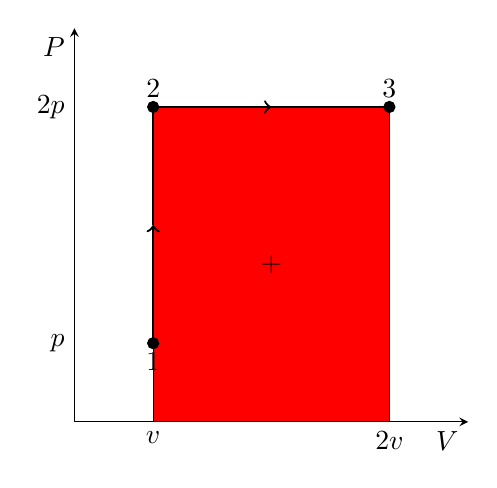
\begin{tikzpicture}
 \draw[stealth-stealth] (0,5) node[below left]{$P$} |- (5,0) node[below left]{$V$};
\filldraw[fill=red] (1,0) rectangle (4,4);
\filldraw (1,1) circle (2pt);
\filldraw (4,4) circle (2pt);
\filldraw (1,4) circle (2pt);

\draw[thick,->] (1,4) -- (2.5,4);
\draw[thick] (2.5,4) -- (4,4);
\draw[thick,->] (1,1) -- (1,2.5);
\draw[thick] (1,2.5) -- (1,4);

\node[above] at (1,4) {$2$};
\node[above] at (4,4) {$3$};
\node[below] at (1,1) {$1$};

%\draw[dashed] (0,4) -- (1,4);
%\draw[dashed] (0,1) -- (1,1);
%\draw[dashed] (1,0) -- (1,1);
%\draw[dashed] (4,0) -- (4,1);

\node[below] at (4,0) {$2v$};
\node[below] at (1,0) {$v$};
\node[left] at (0,1) {$p$};
\node[left] at (0,4) {$2p$};

\draw (2.5,2) node {$+$};
\end{tikzpicture}
\end{center}

And from $3$ back to $1$, the area below the curve represents work that we do \textbf{on} the gas, or the gas doing \textbf{negative} work:

\begin{center}
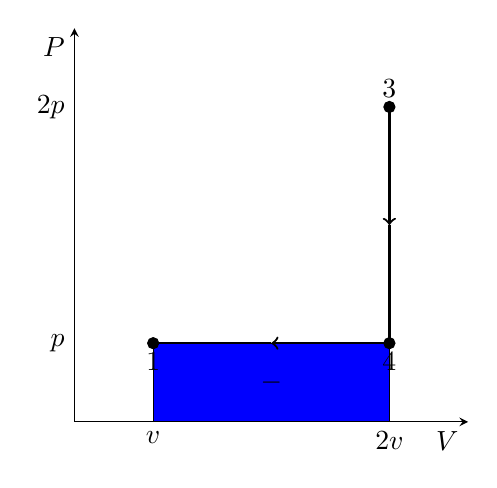
\begin{tikzpicture}
 \draw[stealth-stealth] (0,5) node[below left]{$P$} |- (5,0) node[below left]{$V$};
 \filldraw[fill=blue] (1,0) rectangle (4,1);
\filldraw (1,1) circle (2pt);
\filldraw (4,1) circle (2pt);
\filldraw (4,4) circle (2pt);

\draw[thick,->] (4,4) -- (4,2.5);
\draw[thick] (4,2.5) -- (4,1);
\draw[thick,->] (4,1) -- (2.5,1);
\draw[thick] (2.5,1) -- (1,1);


\node[above] at (4,4) {$3$};
\node[below] at (4,1) {$4$};
\node[below] at (1,1) {$1$};

%\draw[dashed] (0,4) -- (1,4);
%\draw[dashed] (0,1) -- (1,1);
%\draw[dashed] (1,0) -- (1,1);
%\draw[dashed] (4,0) -- (4,1);

\node[below] at (4,0) {$2v$};
\node[below] at (1,0) {$v$};
\node[left] at (0,1) {$p$};
\node[left] at (0,4) {$2p$};
\draw (2.5,0.5) node {$-$};
\end{tikzpicture}
\end{center}

Therefore, over the whole cycle, the net work that the gas/heat engine does for us is just the sum of the two parts:

\begin{center}
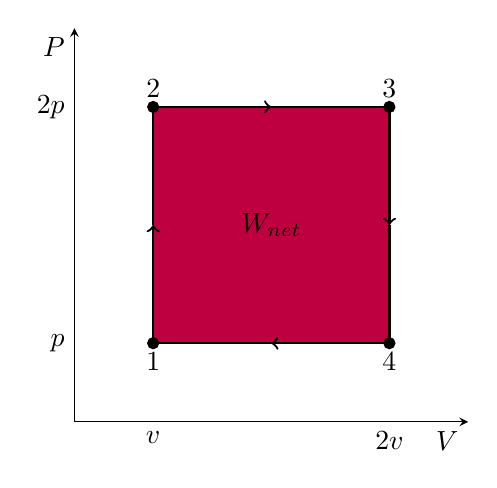
\begin{tikzpicture}
 \draw[stealth-stealth] (0,5) node[below left]{$P$} |- (5,0) node[below left]{$V$};
\filldraw[fill=purple] (1,1) rectangle (4,4);
\filldraw (1,1) circle (2pt);
\filldraw (4,1) circle (2pt);
\filldraw (4,4) circle (2pt);
\filldraw (1,4) circle (2pt);

\draw[thick,->] (1,4) -- (2.5,4);
\draw[thick] (2.5,4) -- (4,4);
\draw[thick,->] (4,4) -- (4,2.5);
\draw[thick] (4,2.5) -- (4,1);
\draw[thick,->] (4,1) -- (2.5,1);
\draw[thick] (2.5,1) -- (1,1);
\draw[thick,->] (1,1) -- (1,2.5);
\draw[thick] (1,2.5) -- (1,4);

\node[above] at (1,4) {$2$};
\node[above] at (4,4) {$3$};
\node[below] at (4,1) {$4$};
\node[below] at (1,1) {$1$};

%\draw[dashed] (0,4) -- (1,4);
%\draw[dashed] (0,1) -- (1,1);
%\draw[dashed] (1,0) -- (1,1);
%\draw[dashed] (4,0) -- (4,1);

\node[below] at (4,0) {$2v$};
\node[below] at (1,0) {$v$};
\node[left] at (0,1) {$p$};
\node[left] at (0,4) {$2p$};
\draw (2.5,2.5) node {$W_{net}$};
\end{tikzpicture}
\end{center}
So in our case, the work the engine does for us is simple; we simply calculate the area of the square, which is just $pv$! Easy! Note that with more complicated looking heat engines (say, with isothermal or adiabatic curves) we might need to be more clever (and either use the formulas we derived\footnote{Which are at heart the same thing as the area argument, because we got those via integration}, or tricks with the first law of thermodynamics and the definition of energy change $\Delta E = nc_v\Delta T$). Of course, there was nothing stopping you from applying those isobaric process work formulas to solve this problem, either. You would find you get an identical result! \\
To figure out the heat that goes in/out of the engine during each process, we can use the formulas that we have derived. Let's start with the heat from $1 \rightarrow 2$. Here, the gas is being isochorically heated, so we know that we are adding heat into the system. We know that its an isochoric process, so there's no work that's done; hence, the only energy change we look at is the heat. Therefore, we have \[ Q_{1\rightarrow 2} = \Delta E  = nc_v \Delta T \]
The temperature difference between $1$ and $2$ is just:
\[\Delta T = T_2 -T_1 = \frac{2pv}{R} - \frac{pv}{R} = \frac{pv}{R} \] 
And for a monoatomic gas, we know that the constant volume heat capacity $c_v$ is:
\[ c_v = \frac{\chi}{2}R = \frac{3}{2}R \]
So therefore the heat that we put in during the $1 \rightarrow 2$ process is:
\[Q_{1\rightarrow 2} = \frac{3}{2}R\frac{pv}{R} = \frac{3}{2}pv \]
Now let's consider the heat flow in the $2 \rightarrow 3$ process. We have isobaric expansion, so we know that we'll have to be putting in heat in order to make that happen, and that heat will have value (from our previous derivation):
\[Q = nc_p\Delta T\]
The temperature difference between $2$ and $3$ can be calculated as:
\[\Delta T = T_3 -T_2 = \frac{4pv}{R} - \frac{2pv}{R} = \frac{2pv}{R} \] 
And the constant pressure heat capacity is:
\[c_p = c_v + R = \frac{3}{2}R + R = \frac{5}{2}R \]
So the heat that we put in during the $2 \rightarrow 3$ process is:
\[Q_{2\rightarrow 3} = \frac{5}{2}R\frac{2pv}{R} = 5pv \]
I'll leave the heat flow for segments $3 \rightarrow 4$ and $4 \rightarrow 1$ for you! However, for both of those last two segments, heat is coming out of the gas (rather than us putting heat into it) so we have everything we need to calculate the efficiency of the heat engine. We have that:
\[Q_{\text{in}} = Q_{1 \rightarrow 2} + Q_{2 \rightarrow 3} = \frac{3}{2}pv + 5pv = \frac{13}{2}pv \]
And the total work done is just $pv$, so the efficiency of our square heat engine is:
\[ \eta = \frac{W_{net}}{Q_{in}} = \frac{pv}{\frac{13}{2}pv} = \frac{2}{13} \approx 15 \% \]
Wow, our cute boxy heat engine turns out to be pretty crummy at its job. It's only 15\% efficient at converting heat into work. Fortunately, not all heat engines are as bad; we'll introduce a much more efficient heat engine in the next section!

\subsubsection{The Carnot Engine}
The Carnot engine is more than just an engine. Its a limit on the efficiency of real-world thermodynamic processes, and was used to develop the first notions of entropy. That being said, like the example above the Carnot engine is a four step cycle.
\begin{center}
            \begin{tikzpicture}[
          dot/.style = {draw,fill,circle,inner sep=1pt},
          arrow inside/.style = {postaction=decorate,decoration={markings,mark=at position .55 with \arrow{>}}}
          ]
          %\draw[<->] (0,6) node[above right] {$P$} |- (6,0) node[right] {$V$};
          %\draw[->] (0,0) node[above] {$P$} %|- (6,0) node[right] {$V$};
 \draw[stealth-stealth] (0,6) node[below left]{$P$} |- (6,0) node[below left]{$V$};
          \node[dot,label={right:$2$}] (@b) at (4.5,4) {};
          \node[dot,label={left:$1$}] (@a) at (1,4.5) {};
          \node[dot,label={below left:$4$}] (@d) at (1.5,1.5) {};
          \node[dot,label={right:$3$}] (@c) at (5,1) {};
          \draw[fleche={0.5:black} ] (@a) to[looseness=.7,bend right=20] (@b);
          \draw[fleche={0.5:black} ] (@b) to[looseness=.7,bend right=20] (@c);
          \draw[fleche={0.5:black} ] (@c) to[looseness=.7,bend left=20] (@d);
          \draw[fleche={0.5:black} ] (@d) to[looseness=.7,bend left=20] (@a);
        \end{tikzpicture}

\end{center}
If we start at state $1$ in the diagram, the engine first undergoes an isothermal expansion to state $2$, while in contact with the hot heat bath. It then undergoes an adiabatic expansion to state $3$ in contact with no heat bath. This is followed by an isothermal compression to state $4$, which occurs while in contact with a cool heat bath. Finally, the engine undergoes an adiabatic compression to return to state $1$. Note that since the processes $1 \rightarrow 2$ and $3 \rightarrow 4$ are isothermal, the engine has only two temperatures. States $1$ and $2$ are at a high temperature ($T_H$), and states $3$ and $4$ are at a low temperature ($T_C)$. \\
While the optional derivation will be given in the next section, you will want to know that the efficiency of the Carnot engine is given by:
\begin{equation}
    \eta = 1 -\frac{T_C}{T_H}
\end{equation}
Where $T_C$ is the coldest/minimum temperature in the cycle and $T_H$ is the hottest/maximum temperature in the cycle. A brief fact about the maximum and minimum temperatures of the heat engine; often these two parameters are given by the ambient temperature and the combustion temperature of the gas in the engine, respectively. This means that if you were to put a Carnot engine inside of your car (though I'm about to tell you why you can't do that in a few sentences), you would find that during the winter your car will run more efficiently than during the summer! Alternatively, if you were to use a gas medium with a higher combustion temperature, you would see a similar effect.\\
One surprising fact: The Carnot efficiency is the maximum possible efficiency attainable by a heat engine\footnote{An interesting consequence of this is that your heat engine can only be 100\% efficient if it's a Carnot engine, and the lowest temperature is $T_C=0$, or the maximum temperature is $T_H = \infty$. Not very realistic either way.}. This isn't just me trying to challenge you to think of something that could be better; it's actually a theorem, and a consequence of the extremely fundamental second law of thermodynamics, which we will explore in depth in the next section. Unfortunately for the world, a truly isothermal process takes an infinitely long time (we'll explore this more in the next section as well). This means that while the Carnot engine might be the most energy efficient, its power output (i.e. the work it does divided by the time it takes) is zero. So unfortunately, you won't be installing a Carnot engine into your car anytime soon..
\subsubsection{(Optional) Deriving the Carnot Efficiency}
Deriving the efficiency of a Carnot engine is difficult, but doable with the knowledge we have so far. I'd suggest you take a shot at it before looking at this section. \\
I'll label the different states of the Carnot cycle as in the diagram above. The efficiency of a heat engine $\eta$ is defined as
\begin{equation*}
    \eta = \frac{W}{Q_{in}}
\end{equation*}
the ratio of the total work done by the system and the heat put into it. From the first law of thermodynamics, we know that $\Delta E = Q - W$, where $W$ is the work done by the system. Since this process ends in the same state it started, we can infer that $\Delta E = 0$, so $Q = W$. Therefore, we get that $W = Q_{in} - Q_{out}$. So we have that
\begin{equation*}
    \eta = 1 - \frac{Q_{out}}{Q_{in}}
\end{equation*}
Heat only flows out of the system from states $c$ to $d$, and only flows into the system from states $a$ to $b$. Both processes are isothermal, so we get
\begin{equation*}
    \eta = 1 - \frac{-P_{3}V_{3}\ln{\Big(\frac{V_4}{V_3}\Big)}}{P_{1}V_{1}\ln{\Big(\frac{V_2}{V_1}\Big)}}
\end{equation*}
To be honest I am hand-waving the signs a bit here, so take some time to make sure you understand them. If you get stuck, remember that in this case positive heat flow is into the system and that the natural logarithm of a number less than one is negative. Anyways, since $T_c$ is the temperature of the low-temperature heat bath and $T_a$ is the temperature of the high-temperature heat bath, I can substitute temperature into the equation using ideal gas law to get
\begin{equation*}
    \eta = 1 - \frac{T_{C}\ln{\Big(\frac{V_3}{V_4}\Big)}}{T_{H}\ln{\Big(\frac{V_2}{V_1}\Big)}}
\end{equation*}
Now all that remains is to show that $\frac{V_2}{V_1} = \frac{V_3}{V_4}$. I'll leave that part to you in one of the questions below. Once you do get this result, you can use it to cancel the logarithms, leaving the equation as
\begin{equation*}
    \eta = 1 - \frac{T_C}{T_H}
\end{equation*}
\subsection{Practice Problems}
\begin{enumerate}
\item If we think back to the ideal gas law, a term that we could add to make it more general (applicable to non-ideal gases) is to add a term correcting for molecular interactions. Doing so, we get the equation:
\begin{equation}
    \label{eqn:(33)}
    \left(P+a\frac{n^2}{V^2}\right)V = nRT
\end{equation}  
where $a\frac{n^2}{V^2}$ is the interaction term. Note that if we also add an $-nb$ term to the volume to account for the size of the molecules, we end up with the very general Van der Waals equation:
\begin{equation}
    \left(P+a \frac{n^{2}}{V^{2}}\right)\left(V-n b\right)=n R T
\end{equation}
But for the purposes of this question, let's assume $b=0$ to make our lives easier.
\begin{enumerate}
    \item Manipulate the equation \ref{eqn:(33)} to obtain pressure as a function of temperature, volume, and amount of gas.
    \item Suppose that I isothermally compress the gas given in equation \ref{eqn:(33)} from $V_1$ to $V_2$. How much work do I do on the gas?
\end{enumerate}

\item For each of the 4 (8) processes of isochoric heating, isochoric cooling, isobaric expansion, isobaric compression, isothermal expansion, isothermal compression, adiabatic expansion, and adiabatic compression, consider:
    \begin{enumerate}
        \item Is work done on/done by the gas, or is it zero?
        \item Does heat flow into or out of the gas, or is it zero?
        \item Does the temperature of the gas increase, decrease, or stay the same?
    \end{enumerate}
\item Consider the following heat engine, composed of 10 moles of monoatomic gas, below:
\begin{center}
    \begin{tikzpicture}
    \begin{axis}[
        axis x line=bottom,
        axis y line=left,
        xmin=0, xmax=10,
        ymin=0, ymax=10,
%        % (made labels more common)
%        % (because of the "sketch" type of the plot these should not be needed)
%        xlabel={Volume $(\mathrm{m}^3)$},
%        ylabel={Pressure (Pa)},
        % (changed ticks + labels to normal ticks instead of extra ticks)
        xtick={3,6},
        xticklabels={$2$,$4$},
        ytick={1.5,6},
        yticklabels={$5$,$15$},  % <-- (changed order of entries)
    ]
        % fill the area below the curve
        % (draw it first, so it is below everything else)


        % draw the dashed lines
        % (using two different approaches)
        \addplot [dashed,domain=0:3,samples=2] {6};
        \addplot [dashed,domain=0:3,samples=2] {1.5};

        \draw [dashed,thin] (axis cs:6,1.5) -- (axis cs:6,0);
        \draw [dashed,thin] (axis cs:3,1.5)   -- (axis cs:3,0);

        % now draw the curve
        \draw [
            fleche={0.55:black}              % <-- added
        ] (axis cs:3,6) to
            % store start and end coordinates
            coordinate [pos=1] (start)
            coordinate [pos=0] (end)
        (axis cs:6,1.5);
        \draw[fleche={0.55:black}] (axis cs:6,1.5) to (axis cs:3,1.5);
        \draw[fleche={0.5:black}] (axis cs:3,1.5) to (axis cs:3,6);

        % draw start and end point
        \fill [radius=2pt]
            (start) circle[]
            (end)   circle[];
        \filldraw[fill=black] (axis cs: 3,1.5) circle (2pt);
    \end{axis}
        \node[below] at (6.5,0) {$V (m^3)$};
        \node[left] at (0,5.5) {$P (kPa)$};
        \node[above] at (2.05,3.5) {$3$};
        \node[right] at (4.25,0.9) {$1$};
        \node[left] at (2.1,1.15) {$2$};
\end{tikzpicture}
\end{center}
\begin{enumerate}
    \item What is the net change in the internal energy of the heat engine after one cycle?
    \item What is the work done by the heat engine in one cycle? (in kiloJoules... note that $1\textrm{Pa}*1\textrm{m}^3 = 1\textrm{J}$)
    \item What is the net heat flow of the heat engine in one cycle? (in kiloJoules)
    \item Solve for the temperature (in Kelvin) at each of the three points.
    \item For each step, determine the work done by the engine, and how much heat flows into/out of the engine. 
\end{enumerate}
\item Consider the following heat engine, composed of monoatomic gas. Treat the process $3 \rightarrow 1$ as isothermal.
\begin{center}
    \begin{tikzpicture}
    \begin{axis}[
        axis x line=bottom,
        axis y line=left,
        xmin=0, xmax=10,
        ymin=0, ymax=10,
%        % (made labels more common)
%        % (because of the "sketch" type of the plot these should not be needed)
%        xlabel={Volume $(\mathrm{m}^3)$},
%        ylabel={Pressure (Pa)},
        % (changed ticks + labels to normal ticks instead of extra ticks)
        xtick={3,6},
        xticklabels={$V_0/2$,$V_0$},
        ytick={1.5},
        yticklabels={$P_0$},  % <-- (changed order of entries)
    ]
        % fill the area below the curve
        % (draw it first, so it is below everything else)


        % draw the dashed lines
        % (using two different approaches)
        \addplot [dashed,domain=0:3,samples=2] {1.5};

        \draw [dashed,thin] (axis cs:6,1.5) -- (axis cs:6,0);
        \draw [dashed,thin] (axis cs:3,1.5)   -- (axis cs:3,0);

        % now draw the curve
        \draw [
            fleche={0.55:black}              % <-- added
        ] (axis cs:3,6) to [bend right = 30]
            % store start and end coordinates
            coordinate [pos=1] (start)
            coordinate [pos=0] (end)
        (axis cs:6,1.5);
        \draw[fleche={0.55:black}] (axis cs:6,1.5) to (axis cs:3,1.5);
        \draw[fleche={0.5:black}] (axis cs:3,1.5) to (axis cs:3,6);

        % draw start and end point
        \fill [radius=2pt]
            (start) circle[]
            (end)   circle[];
        \filldraw[fill=black] (axis cs: 3,1.5) circle (2pt);
    \end{axis}
        \node[below] at (6.5,0) {$V$};
        \node[left] at (0,5.5) {$P$};
        \node[above] at (2.05,3.5) {$3$};
        \node[right] at (4.25,0.9) {$1$};
        \node[left] at (2.1,1.15) {$2$};
\end{tikzpicture}
\begin{enumerate}
    \item What is the ratio of the temperatures between point $3$ and point $1$?
    \item Solve for the pressure at point $3$ in terms of $P_0$ and $V_0$
    \item Mark the highest temperature $T_H$ and the lowest temperature $T_C$ on the graph. 
    \item Solve for the efficiency of the heat engine. Your answer should not depend on $P_0$, $V_0$, or the amount of gas in the heat engine. (Note: Solving for the efficiency is quite a bit more difficult than the other parts; a partial solution of the work and heat done during certain steps would be a good partial solution.)
\end{enumerate}
\end{center}
\item Question 4 again, except this time treat process $3 \rightarrow 1$ as adiabatic (Note that part (d) is \textit{quite} difficult).
\item Use what you know of adiabatic and isothermal processes to finish deriving the Carnot efficiency.

\end{enumerate}
\newpage
\section{Entropy}
Entropy is central to the second and third laws of thermodynamics, as well as understanding the spontaneity of processes. It's a concept you'll see appear not only in physics, but in chemistry and biology as well.

\subsection{Types of Systems}
Just before we define our notion of this mysterious "entropy", it will help to define what different kinds of systems mean. An \textbf{Open system} is one in which both matter and energy can be exchanged with its environment. A \textbf{Closed system} is a system where energy can be exchanged with the environment, but no matter. Finally, an \textbf{isolated} system is where neither matter nor energy can be exchanged with the environment. \\
As a quick example, suppose my system is a half cup of water. If I leave the top of the cup open, it's an open system as the water molecules can evaporate and leave the cup. If I close the top of the cup, then it's a closed system as I can still give energy to the cup (say, by heating it in a microwave) even if the water molecules can't escape from it. If the cup is perfectly insulated and closed off, then its an isolated system as neither matter nor energy can enter or exit the cup. With this in mind, let's proceed with the most mindbending concept of this unit!
\subsection{The Classical Definition of Entropy}
Jumping right into things, entropy, for large systems, can be defined as
\begin{equation}
    dS=\frac{\delta Q_{rev}}{T}
\end{equation}
Where $dS$ is the change in entropy, $\delta Q_{rev}$ is heat reversibly flowing to/from a system, and $T$ is the temperature of the system. Just stating it right here, this equation probably seems to make \textbf{no} sense whatsoever, so let's step back a bit to build up to it.
\subsubsection{Reversable Processes}
First we need to talk about reversible processes. A reversible process, broadly speaking, is one that can spontaneously take place in both directions. Let's take a look at an example: say we have two large closed chambers of gas in an isolated system. The only way they can interact is via heat flow.
\begin{figure}[h!]
    \centering
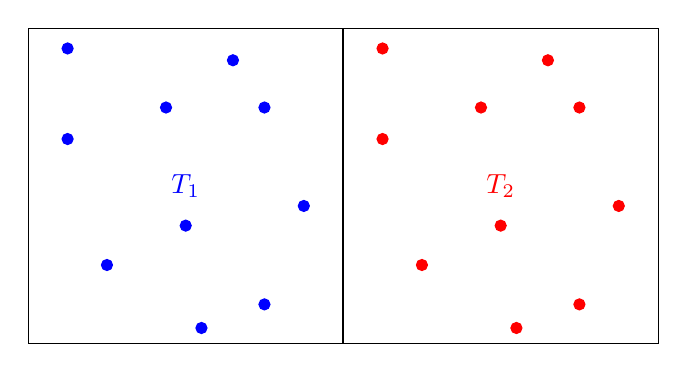
\begin{tikzpicture}
\draw[draw = black] (0,0) rectangle (8,4);
\draw[thick] (4,0) -- (4,4);
\draw[text=blue] (2,2) node {$T_1$};
\draw[text=red] (6,2) node {$T_2$};
\draw[fill=blue, draw=blue] (1,1) circle (2pt);
\draw[fill=blue, draw=blue] (3,0.5) circle (2pt);
\draw[fill=blue, draw=blue] (0.5,2.6) circle (2pt);
\draw[fill=blue, draw=blue] (2.6,3.6) circle (2pt);
\draw[fill=blue, draw=blue] (3.5,1.75) circle (2pt);
\draw[fill=blue, draw=blue] (1.75,3) circle (2pt);
\draw[fill=blue, draw=blue] (2,1.5) circle (2pt);
\draw[fill=blue, draw=blue] (2.2, 0.2) circle (2pt);
\draw[fill=blue, draw=blue] (3,3) circle (2pt);
\draw[fill=blue, draw=blue] (0.5, 3.75) circle (2pt);
\draw[fill=red, draw=red] (5,1) circle (2pt);
\draw[fill=red, draw=red] (7,0.5) circle (2pt);
\draw[fill=red, draw=red] (4.5,2.6) circle (2pt);
\draw[fill=red, draw=red] (6.6,3.6) circle (2pt);
\draw[fill=red, draw=red] (7.5,1.75) circle (2pt);
\draw[fill=red, draw=red] (5.75,3) circle (2pt);
\draw[fill=red, draw=red] (6,1.5) circle (2pt);
\draw[fill=red, draw=red] (6.2, 0.2) circle (2pt);
\draw[fill=red, draw=red] (7,3) circle (2pt);
\draw[fill=red, draw=red] (4.5, 3.75) circle (2pt);
\end{tikzpicture}
    \caption{The wonderful box with two closed sections.}
\end{figure}
\\ If one side is at a higher temperature than the other, then we intuitively know that heat will flow from the hot side to the cool side. But what happens if their temperatures are the same? The short answer is: absolutely nothing. But it's an exciting nothing! Let's dig even deeper. \\
\newline
Say we were to zoom in extremely close on that boundary between the two sides of the box. What would we see? Unsurprisingly, a lot of very small particles hitting a very large wall. However, we know that in order for heat to flow across that barrier, the particles need some way of transferring their energy across the wall. How could they do it? Well, there's two possible ways. The first is radiation, which we'll pretend doesn't exist (it makes our lives much easier, and isn't a terrible assumption). The other is through the wall itself. That is, when a particle collides with the wall, a bit of its kinetic energy goes into the wall, which then gives it up to a particle colliding on the other side.
\newline\newline
Here's the key though: particles on both sides of the wall do this, regardless of the temperature difference. Even if we had the right side of the box at $10^{20}\mathrm{K}$ \footnote{Actually at a temperature this high there would be no box.} and the left side at $100\mathrm{K}$, some particles from the left side of the box would hit the wall and give up some energy to the right side. It's just that particles on the right side of the box are
\begin{enumerate}
    \item Giving up way more energy when they hit the wall.
    \item Hitting the wall far more frequently.
    \item And/or both!
\end{enumerate}
So the \textit{net} transfer of energy is from the right side of the box to the left. In a situation like this, where there is a spontaneous net transfer of energy, we'd say that said process is irreversible. However, if the temperature in the box was the same at both sides, we'd expect no net heat transfer to take place. Therefore, we could conclude that
\begin{itemize}
    \item Both sides give up the same amount of energy per collision on average.
    \item Both sides have the same frequency of collision.
\end{itemize}
This is where the symbol $\delta$ comes in. As the profs may or may not have mentioned in lecture, it means a \textit{very very very} small change. Which, it so happens, is the perfect way to describe the change in energy/temperature each side of the box has when one collision occurs. So we have a very small heat flow, and essentially constant temperature. Furthermore we can see that this tiny flow of heat has an equal chance of happening in both directions, and will. Hence, its reversible!
\newline\newline
So now that we have a better idea of what a reversible process is, we can better understand what entropy is. As a quick reminder, we said above that
\begin{equation*}
    dS=\frac{\delta Q_{rev}}{T}
\end{equation*}
With our newfound knowledge we can say that this says: the change in entropy of a system ($dS$) in a \textit{reversible} heat transfer is \textit{directly} proportional to the amount of heat transferred into the system and \textit{inversely} proportional to the temperature of the system.\footnote{Some of you may wonder if this definition still can be applied when the heat transfer is irreverisible. It can, but the equality is replaced by in inequality $dS > \frac{dQ}{T}$. So if you wanted the most general definition would be $dS \geq \frac{dQ}{T}$.}
\newline\newline
We say above that our tiny reversible processes happen between two systems at the same (constant) temperature. Here's the issue though, and the one that causes us to define all our reversible processes (and entropy) as infinitesimals: no reversible process actually exists on a macroscopic scale.
\newline\newline
As an example of why this is, let's take a look at a process that is theoretically reversible, but isn't actually reversible. Say we have a container of a gas with a piston on one face, but insulated such that it cannot exchange heat (or molecules) with its environment. However, it is connected to a neighbouring infinitely large heat bath, where it can exchange heat with (but not molecules). 
\begin{figure}[h!]
\centering
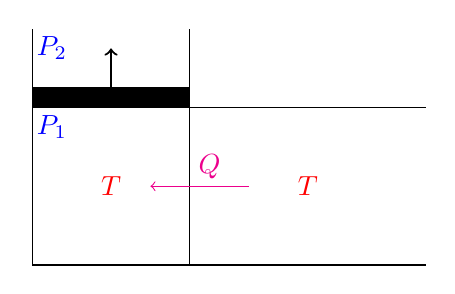
\begin{tikzpicture}
\draw[draw=black] (0,0) rectangle (2,2);
\draw[fill = black] (0,2) rectangle (2,2.25);
\draw (0,2) -- (0,3);
\draw (2,2) -- (2,3);
\draw (2,2) -- (5,2);
\draw (2,0) -- (5,0);
\draw[->, thick] (1, 2.25) -- (1, 2.75);
\draw[text=blue] (0.25,1.75) node {$P_1$};
\draw[text=blue] (0.25, 2.75) node {$P_2$};
\draw[text=red] (1,1) node {$T$};
\draw[text=red] (3.5,1) node {$T$};
\draw[magenta, ->] (2.75,1) -- (1.5,1);
\draw[text=magenta] (2.25, 1.25) node {$Q$};
\end{tikzpicture}
\caption{Piston with infinite heat bath to the right.}
\end{figure}
In this situation, we have that $P_{1}>P_{2}$, so the piston will undergo an expansion. Since the heat bath beside it will keep it at the same temperature, the expansion will be isothermal. So since the temperature of the two sides of the piston/heat bath barrier is constant and equal, the heat transfer across it reversible right? Well, not quite. And it has to do with the idea that a perfectly isothermal process doesn't exist either.
\newline\newline
To figure out why, let's break down what happens step by step. Initially, both the gas and the heat bath are at the same temperature, so no net heat flow between them. However, the pressure inside the piston is greater than the pressure outside. So the piston expands. When it does this, it does work on the environment, and loses energy. This in turn causes its temperature to fall. Its temperature dropping causes heat to flow spontaneously across from the heat bath, until the gas returns to its original temperature. Rinse, repeat until the internal and external pressures are equal.
\newline\newline
So we can see that during an isothermal process, the temperature isn't quite constant. However, if we do this process \textit{very} slowly, the heat flow will manage to restore the temperature so quickly (or to put it another way, heat will flow into the system much faster than the system does work) that the temperature be \textit{almost} constant the whole time. This is what we really mean by an isothermal process. It's also why entropy is defined infinitesimally, since we approximate that each of our tiny expansion steps of the piston happen at constant temperature.
\newline\newline
That being said, imagining an ideal, isothermal process is extremely useful, especially at small time scales. It allows us to derive the following formula for the change in entropy:
\begin{equation}
    \label{eqn:(36)}
    \Delta S=n{c_{v}}\ln{\frac{T_1}{T_0}} + nR\ln{\frac{V_1}{V_0}}
\end{equation}
Here, $n$ is the number of mols of gas, $c_v = \frac{\chi}{2}R$ as we defined earlier (for $\chi$ degrees of freedom and the gas constant $R$), $T_0$ and $T_1$ are the initial and final temperatures, and $V_0$ and $V_1$ are the initial and final volumes. First, the change in entropy depends only on the initial and final states of the system (i.e. the final and initial temperatures and volumes), not the path between those states! So \textbf{entropy is function of state}.
\newline\newline
The second thing you should notice is that entropy of a system is dependent on the volume, an \textit{extensive} quantity. Therefore, \textbf{entropy is an extensive quantity}.

\subsubsection{(Optional) Derivation of the Sackur–Tetrode Equation}
Equation \ref{eqn:(36)} as shown above is actually a version of the Sackur-Tetrode equation, which gives the entropy of a monoatomic ideal gas in full. While the derivation of the full equation is far, far out of the scope of this course\footnote{You may consult Wikipedia if you want to see the full equation}, equation \ref{eqn:(36)} can totally be derived with the things we have learned. This derivation is more for your curiousity than anything, and you do already have all the tools required to derive it (so if you're keen, give it a shot!). We start from the definition of entropy (for a reversible heat transfer):
\begin{align*}
    dS = \frac{dQ}{T}
\end{align*}
Now, we consider the first law of Thermodynamics:
\[
    dE = dQ+dW
\]
So let us substitute $dQ = dE-dW$ to obtain:
\[ dS = \frac{dE-dW}{T} = \frac{dE}{T}-\frac{dW}{T}
\]
We apply the (at this point, well-acquainted) formula for change in energy:
\[dE = nc_vdT \]
And we hence obtain:
\[ dS = \frac{nc_vdT}{T} - \frac{dW}{T} \]
We may now use the ideal gas law:
\[T = \frac{PV}{nR} \]
As well as the definition of work:
\[dW = -PdV \]
Substituting these in, we obtain:
\[ dS = \frac{nc_vdT}{T} + \frac{PdV}{\frac{PV}{nR}}\]
Which simplifies to:
\[dS = nc_v\frac{dT}{T} + nR\frac{dV}{V} \]
Now, we integrate from an initial state to a final state (in other words, from a initial entropy/temperature/volume $S_0,T_0,V_0$ to a final entropy/temperature/volume $S_1,T_1,V_1$:
\[\int_{S_0}^{S_1} dS = \int_{T_0}^{T_1}nc_v\frac{dT}{T} + \int_{V_0}^{V_1}nR\frac{dV}{V} \]
Performing the integration, we obtain:
\[ \left.S \right|_{S_0}^{S_1} = nc_v \left. \ln(T) \right|_{T_0}^{T_1} + nR \left. \ln(V) \right|_{V_0}^{V_1} \]
\[ \Delta S = nc_v\ln\left(\frac{T_1}{T_0}\right) + nR \ln\left(\frac{V_1}{V_0}\right) \]
Which is the desired result. 
\subsubsection{\texorpdfstring{The 2\textsuperscript{nd} Law of Thermodynamics}{The 2nd Law of Thermodynamics}}
Now that we've gotten through all of that, we can finally talk about the second law of thermodynamics. It states that:
\begin{center}
    \textbf{The entropy of an isolated system cannot decrease, and will increase if possible.}
\end{center}
Or, put another way, an isolated system will always progress towards a state of maximum entropy. Say you have an isolated system with a few closed systems inside of it. It just so happens that the maximum entropy of the entire isolated system is reached when all the closed systems inside of it are at the same temperature! (The exact reason of why this is the maximum entropy state will be revealed very soon!) This gives us a reason why heat flows from hot to cold, to maximize entropy.
\newline\newline
I'm going to backtrack a bit here to make a very important point. The proper definition of a reversible process is based on the second law of thermodynamics. A reversible process is one in which the entropy of the isolated system does not change. Since entropy is a function of state, running this process in reverse would also result in no entropy change. So, the second law of thermodynamics allows the process to run in both directions. If the process instead saw the entropy of the system increase, running it in reverse would see the entropy of the system decrease, which violates the second law of thermodynamics. The only truly isolated system is the entire universe\footnote{Depending on who you ask, maybe not.}, so a process is reversible if and only if it does not change the entropy of the universe.
\newline\newline
Using this idea of reversibility, we can see that no macroscopic process be truly reversible. For an isothermal process we can say $\Delta S \approx \frac{Q}{T}$\footnote{Ask the chemists!}, which clearly isn't zero unless nothing happens at all. Hence, it's not reversible in an isolated system.
\newline\newline
However, we still have some gaps in our understanding regarding entropy. For example, if right now I gave you the current state of a system, you couldn't calculate it's entropy! We've only characterized the \textit{change} in entropy. That seems silly, so lets fix that.

\subsubsection{\texorpdfstring{The 3\textsuperscript{rd} Law of Thermodynamics}{The 3rd Law of Thermodynamics}}
The third law of thermodynamics is that fix. It states that
\begin{center}
    \textbf{As the temperature of a system tends towards absolute zero, the entropy of the system tends towards a finite value.}
\end{center}
Great! That means that using zero as our reference point, we can calculate the entropy of the system at any other state.

But here's the thing (thing might be the 956\textsuperscript{th} time I've said this). We've figured our \textit{how} entropy behaves, and can use it to predict the future behaviour of the system. But we seem no closer to figuring out \textit{what} entropy is or \textit{why} it behaves the way it does. Luckily, someone else has already figured that out quite a while ago!
%\subsubsection{(TODO) The Carnot Engine, Revisited}
%Before moving onto the statistical definition of entropy, let's answer a question about Carnot engines that might have arose as we learned about entropy; 
%\textit{How can Carnot Engines run reversibly if macroscopic processes are not truly reversible?}The answer is twofold. First, as we mentioned before the Carnot process is an idealization. It involves two isothermal steps, and as we've discussed no process is truly isothermal, unless it ran for an infinitely long time. Second, you need to be careful what system your considering when you say a process is reversible. The heat engine has zero change in entropy. However, when it interacts with its surroundings it inevitably changes the surrounding's entropy as well. Actually modelling this change in entropy would be fiendishly difficult \textbf{Rio Help I'm not sure this is right}, but we'd expect a high level of idealization to be necessary to actually make it zero, and otherwise for it to be positive. We could try to get around this problem by isolating the engine, but the efficiency of the engine is less than 100\%, so it needs a source of energy outside the system.

\subsubsection{(Optional) The Carnot Efficiency, Revisited}
To finish off this section, I want to show you a neat proof of Carnot's theorem; This theorem tells us that the maximum efficiency of a heat engine is given by $\eta = 1- \frac{T_C}{T_H}$ (the efficiency of the Carnot engine), where $T_C$ is the coldest temperature within the cycle, and $T_H$ is the hottest temperature within the cycle. We will explore in this section how this follows from the second law of thermodynamics. This section is completely optional, and just for your curiosity\footnote{Like seriously, this is completely out of the scope of Science One}, though you have all the tools you need to prove it yourself. To review how a heat engine fundamentally works, it takes in some heat $Q_H$ from a hot reservoir at temperature $T_H$, does some work $W$ with that energy, and then throws away waste heat $Q_C$ into a cold reservoir at temperature $T_C$, before returning to its initial state. This is pictured below:
\begin{center}
    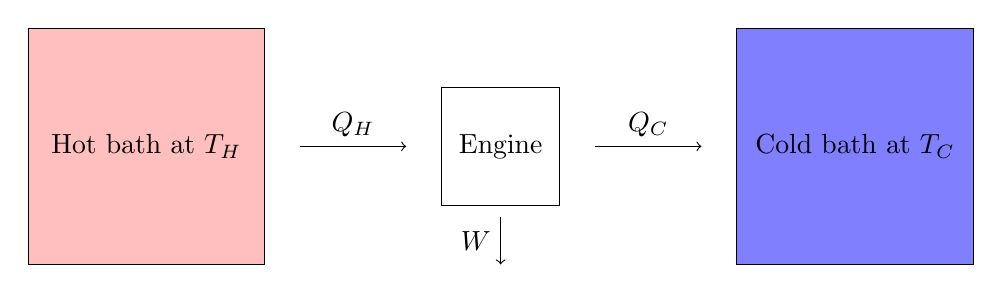
\begin{tikzpicture}[scale=3]
    \filldraw[fill=pink] (0,0) rectangle (1,1);
    \draw (1.75,0.25) rectangle (2.25,0.75);
    \filldraw[fill=blue!50] (3,0) rectangle (4,1);
    \draw[->] (1.15,0.5) -- (1.6,0.5);
    \draw[->] (2.4,0.5) -- (2.85,0.5);
    \draw[->] (2,0.2) -- (2,0);
    \node[above] at (1.375,0.5) {$Q_H$};
    \node[above] at (2.625,0.5) {$Q_C$};
    \node[left] at (2,0.1) {$W$};
    \draw (2,0.5) node {Engine};
    \draw (0.5,0.5) node {Hot bath at $T_H$};
    \draw (3.5,0.5) node {Cold bath at $T_C$};=
    \end{tikzpicture}
\end{center}


Now, let's consider the entropy of the hot reservoir, the engine, and the cold reservoir at the end of one cycle (in other words, we consider the change in entropy of the universe after one cycle). We recall that entropy is a function of state, and therefore at the end of a single cycle, the entropy of the heat engine itself must be the same as when it started. That is, $\Delta S_{engine} = 0$ for one full cycle. By the second law of thermodynamics $dS \geq \frac{Q}{T}$, the entropy of the hot reservoir decreases by the amount of heat $Q_H$ divided by its temperature $T_H$, so the entropy of the hot reservoir decreases by $\Delta S_{hot} \geq \frac{-Q_H}{T_H}$. Conversely, the cold reservoir increases in one cycle by $\Delta S_{cold} \geq \frac{Q_C}{T_C}$ (as it receives $Q_C$ heat at temperature $T_C$. Putting these together, we obtain the change in entropy of the universe for a single cycle:
\[\Delta S_{universe} \geq \frac{Q_C}{T_C} - \frac{Q_H}{T_H} \]
Now, the second law of thermodynamics tells us that the entropy of the universe must increase (or, to phrase it another way, if we treat the two reservoirs and the heat engine as an isolated system, the entropy of the total system must increase. This allows us to conclude that:
\[\Delta S_{universe} \geq \frac{Q_C}{T_C} - \frac{Q_H}{T_H} \geq 0 \]
So we obtain the important inequality:
\[\frac{Q_C}{T_C} - \frac{Q_H}{T_H} \geq 0 \]
Which we can rearrange to obtain:
\begin{equation}
    \label{eqn:(37)}
    \frac{T_H}{T_C} \geq \frac{Q_C}{Q_H}
\end{equation}
Note that to derive inequality \ref{eqn:(37)}, I have made no assumptions whatsoever about what my heat engine actually looks like; this is a completely general statement, based on the amounts of heat gained/lost from the hot/cold reservoirs, and the maximum/minimum hot/cold reservoir temperatures. Now, let us consider out definition of efficiency:
\begin{equation}
    \label{eqn:(38)}
    \eta = \frac{W}{Q_H}
\end{equation}
Where $W$ is the work done by the engine (what we get out), and $Q_H$ is the heat that we inject into the engine in one cycle from the hot reservoir (what we put in). By energy conservation, we find that:
\begin{equation}
    \label{eqn:(39)}
    W = Q_H-Q_C
\end{equation}
This might look like it came out of nowhere, so let's think about it a bit further. Just like entropy, internal energy is also a function of state; the energy something has doesn't care about how that energy got there! With this consideration, since the heat engine returns to the original state at the end of one cycle, just like the entropy change of the heat engine is zero in a single cycle, so must be the total internal energy; in other words, the heat engine must have the same energy it began with. With this consideration, we realize that the sum of the work done on the system and the heat given to the system must be 0, leading to equation \ref{eqn:(39)} above (work this out using the first law of thermodynamics if it's still unclear!). Now, we can substitute equation \ref{eqn:(39)} into equation \ref{eqn:(38)}, giving us:
\begin{align*}
    \eta = \frac{Q_H-Q_C}{Q_H} = 1 - \frac{Q_C}{Q_H}
\end{align*}
And now applying inequality \ref{eqn:(37)}, we have:
\begin{align*}
    1 - \frac{Q_C}{Q_H} \leq 1 - \frac{T_H}{T_C}
\end{align*}
And therefore:
\begin{equation}
    \eta \leq 1 - \frac{T_H}{T_C}
\end{equation}
We have hence proven Carnot's theorem, and can see that for any arbitrary heat engine, the efficiency is bounded by the Carnot efficiency. 

\subsection{The Statistical Definition of Entropy}
Entropy has a more fundamental definition (though that doesn't make the classical definition any less important) rooted in statistics. To understand it, we're going to start of my talking about macrostates and microstates.
\subsubsection{Macrostates and Microstates}
I'll try to define these two words as succinctly as I can.
\begin{itemize}
    \item Macrostate: The state of a system as characterized by quantities that can be measured independent of any one part of the system. Some examples of such quantities would be: Pressure, Volume, and Temperature.
    \item Microstate: The state of a system as characterized by the state of individual components of the system. For example, the exact spacial distribution of particles within a gas.
\end{itemize}
Let's look as a bit more of a concrete example. Say we're looking at a box with 6 particles, divided into two halves.

\begin{figure}[ht!]
    \centering
\begin{tikzpicture}
\draw[draw = black] (0,0) rectangle (6,3);
\draw[dashed] (3,0) -- (3,3);
\draw[fill=red, draw=red] (1,2) circle (2pt);
\draw[fill=blue, draw=blue] (2,2) circle (2pt);
\draw[fill=cyan, draw=cyan] (1.5,1) circle (2pt);
\draw[fill=magenta, draw=magenta] (4,1) circle (2pt);
\draw[fill=orange, draw=orange] (5,1) circle (2pt);
\draw[fill=green, draw=green] (4.5,2) circle (2pt);
\end{tikzpicture}
    \caption{The box with three particles on each side.}
\end{figure}
\phantom{i} \\
\phantom{i} \\
The \textit{macrostate} of this box is something we could say without knowing which particle was where. Without knowing that, all we could say is that each side of the box has three particles. So, the macrostate of the box is three particles on each side. The \textit{microstate} of the box would then be which exact side each particle was on. So for example...

\begin{figure}[ht!]
    \centering
\begin{tikzpicture}
\draw[draw = black] (0,0) rectangle (6,3);
\draw[dashed] (3,0) -- (3,3);
\draw[fill=red, draw=red] (1.5,1.5) circle (2pt);
\draw[fill=blue, draw=blue] (5,1) circle (2pt);
\draw[fill=cyan, draw=cyan] (4.5,1.5) circle (2pt);
\draw[fill=magenta, draw=magenta] (4,2) circle (2pt);
\draw[fill=orange, draw=orange] (4,1) circle (2pt);
\draw[fill=green, draw=green] (5,2) circle (2pt);
\end{tikzpicture}
    \caption{This box has a different number of particles on each side, so it's in as different \textit{macrostate} than the first one.}
\end{figure}
\begin{figure}[ht!]
    \centering
\begin{tikzpicture}
\draw[draw = black] (0,0) rectangle (6,3);
\draw[dashed] (3,0) -- (3,3);
\draw[fill=red, draw=red] (1,2) circle (2pt);
\draw[fill=orange, draw=orange] (2,2) circle (2pt);
\draw[fill=cyan, draw=cyan] (1.5,1) circle (2pt);
\draw[fill=magenta, draw=magenta] (4,1) circle (2pt);
\draw[fill=blue, draw=blue] (5,1) circle (2pt);
\draw[fill=green, draw=green] (4.5,2) circle (2pt);
\end{tikzpicture}
    \caption{This box has the same number of particles on each side, so it's the same \textit{macrostate} as the first one. However, the blue and orange particles have switched sides, making this a different \textit{microstate} than the first box had. Note that two different macrostates of a system cannot share a microstate.}
\end{figure}
\newpage



\subsubsection{The Definition of Entropy}
Now that we know what micro and macro states are, we can define entropy using statistics! In this case, entropy is defined as
\begin{equation}
    \label{eqn:(41)}
    S=k_{b}\ln{\Omega}
\end{equation}

where $\Omega$ is the number of possible microstates within the current macrostate of the system. \\
With a closed system of constant volume, we can characterize macrostates using the temperature of the system, and microstates as the exact distribution of kinetic energies amongst the particles in the system. Using this we can start to see all the parallels between the two different ways of defining entropy.
\begin{enumerate}
    \item At $T=0\textrm{K}$ every particle must have no kinetic energy. So, there's only one possible microstate, and by equation \ref{eqn:(41)} above $S=0$. This is exactly what we'd expect from the third law of thermodynamics, at absolute zero temperature, we obtain that entropy has a constant value\footnote{Note that the third law of thermodynamics does not say a system reaches zero entropy as it approaches zero temperature, as there do exist certain systems where the minimum energy (i.e. low temperature) states are not unique. Therefore, there still can be more than one microstate, and hence nonzero (but still constant) entropy. You don't need to know about these in any kind of detail.}.
    \item If you have two systems (a and b), the amount of microstates in a system including both of them is $\Omega_{a}\Omega_{b}$. Therefore, the total entropy is...
    \begin{align*}
        S_{total}&=k_{b}\ln{\Omega_{a}\Omega_{b}} \\
        &=k_{b}\ln{\Omega_{a}}+k_{b}\ln{\Omega_{b}} \\
        &=S_{1}+S_{2}
    \end{align*}
    Since the total entropy is the sum of the entropy of both systems, entropy is an extensive quantity!
    \item In our example for microstates/macrostates above, the macrostate with the highest number of microstates was the one where each side had three particles (if you don't believe me count them). This analogy applies to two systems that can exchange energy, they have the maximum number of microstates (and therefore entropy) when they share the energy equally (i.e. have the same temperature). 
\end{enumerate}
To close off our discussion of macrostates, microstates, and the statistical definition of entropy, let us consider another concrete example, in the form of the entropy of rolling two dice. Therein, we can consider the macrostate as the sum of the two dice rolls, and the microstates as the particular values we got on each dice (here, we imagine that the dice are unique, in that I can tell them apart from each other). For example, if I rolled the first dice to be 6, and the second dice to be 1, then the microstate could be described with $(6,1)$ and this microstate belongs to the macrostate of $7$. A complete description of all of the macrostates and microstates (as well as the entropy of the macrostate, as defined in this section) is given in the table below, though you may want to work this out for yourself first for practice.

\begin{center}
 \begin{tabular}{|c c c|} 
 \hline
 \textbf{Macrostates} & \textbf{Microstates} & \textbf{Entropy}\\ 
 \hline\hline
 2 & (1,1) & $k_b\ln(1) = 0$\\ 
 \hline
 3 & (1,2),(2,1) & $k_b\ln(2)$ \\
 \hline
 4 & (1,3),(2,2),(3,1) & $k_b\ln(3)$ \\
 \hline
 5 & (1,4),(2,3),(3,2),(4,1) & $k_b\ln(4)$ \\
 \hline
 6 & (1,5),(2,4),(3,3),(4,2),(5,1) & $k_b\ln(5)$ \\
 \hline
 7 & (1,6),(2,5),(3,4),(4,3),(5,2),(6,1) & $k_b\ln(6)$\\
 \hline
 8 & (2,6),(3,5),(4,4),(5,3),(6,2) & $k_b\ln(5)$\\
 \hline
 9 & (3,6),(4,5),(5,4),(6,3) & $k_b\ln(4)$\\
 \hline
 10 & (4,6),(5,5),(6,4) & $k_b\ln(3)$\\
 \hline
 11 & (5,6),(6,5) & $k_b\ln(2)$\\
 \hline
 12 & (6,6) & $k_b\ln(1) = 0$\\
 \hline
\end{tabular}
\end{center}
This example also demonstrates an assumption I implicitly made up until this point: all possible microstates are equally likely to appear (in the last example, unless you had loaded dice, every dice roll would have been equally likely!). This is a very fundamental assumption, so much so that it is called the \textbf{Fundamental Assumption of Statistical Mechanics}. Just to restate it for a more general case (as not every system in the universe is a bunch of dice), it states that every microstate of a system is equally likely and the system on average spends the same amount of time in each of them. We will use this in the next section to conclude our discussion of entropy. 
\subsubsection{The Arrow of Time}
One interesting property of a lot of physics equations is that they are invariant under time reversal; that is, equations like Newton's second law 
\begin{align*}
\vec{F} = m\vec{a}
\end{align*}
can be applied even in cases where time was running in reverse\footnote{Assuming no friction, of course.}. However, it is clear in our immediate experience that a lot of things are not invariant under time reversal. If I were to show you a video of heat flowing from a cold bath of water to a hot bath of water, you would tell me immediately that the video must be playing in reverse. If the laws of physics are supposed to work the same way in either direction, what's going on here?

As we discussed previously, where we see phenomena that only proceed in one time direction, what we are seeing is something go from a low entropy state to a higher entropy state. After the process, by the second law of thermodynamics, we can't go back to the lower entropy state. But this explanation feels a bit unsatisfactory; sure, we've accepted the second law of thermodynamics as a law, but there's still this underlying feeling of "Well, why \textbf{can't} things go back to a lower entropy state?" The statistical definition will allow us to settle this confusion once and for all.

From a statistical viewpoint, what are we saying when a system goes from a low to a high entropy state? Well by the definition of $S = k_b\ln\mathbb{W}$ for the entropy of a macrostate, what we're really saying is that the system moves from a macrostate with a low number of microstates to a high number of microstates. Okay sure, but why? Well let's think back to the fundamental assumption of statistical mechanics that I just outlined a page ago. This assumption tells us that every microstate is equally as likely to appear, and each microstate persists for the same amount of time. Well, if every microstate is equally as likely, then simple notions of probability will tell us that the system at any given point will tend to a macrostate with more microstates.

Let's try to make this a little more concrete with an example. Say I was keeping tracks of 10 numbered cows in a field, separated into a left and right hand side, where the cows were allowed to walk around the field totally randomly. Then, a macrostate of the system could be defined by how many cows were on the left side of the field (where I have 11 microstates, from 0-10 cows on the left side). Now, suppose I start in a configuration where all 10 cows are on the left side of the field. There are a couple ways in which I could arrange the cows in this scenario. However, the macrostate corresponding to 5 cows on the right side and 5 cows on the left side of the field has a lot more microstates; there are a lot more ways I could arrange 5 and 5 cows on either side of the field compared to having all the cows on one side. With this in mind, let's imagine that the cows start all on one side, I walk away from the field, and come back some amount of time later after the cows were free to move around. Since every configuration of cows is equally likely, I would be most likely see a state where the cows were distributed equally on both sides of the field (as we would expect). Probabilistically, the system has evolved from an initial low entropy state (all cows on one side) to a higher entropy state (cows distributed on both sides).

Now, imagine instead of left and right side of a field, we have two containers of gas in thermal contact, which can freely exchange units of energy (which have replaced the cows in this scenario). Although now we have an extremely large number of energy units instead of just 10\footnote{Many 10s of orders of magnitude more...}, the same sort of logic applies; if I start in a macrostate with all of the energy units on one side (i.e. one gas container is very hot, and the other is not), with time, the system will tend to a macrostate of thermal equilibrium (approximately equal thermal energy on either side) as there are so many more microstates for the equilibrium temperature macrostate compared to a macrostate where one side has a lot more energy units than the other. Hence, we have come up with a statistical explanation for why heat tends to flow from hot objects to cold objects!

Note that this analysis reveals something interesting about the second law of thermodynamics; it's very much a statistical law, that tells us that a isolated system is (extremely) likely to tend to a high entropy state. Note that both in the cows and the heat example, there technically is a possibility that the system could temporarily return to a low entropy state (either with all the cows, or all the thermal energy units on one side); its just that this configuration is \textbf{extremely unlikely}. In fact, as we make our system larger and larger, the likelihood that the system could ever return to a low entropy state becomes more and more unlikely, and therefore in the limit of large/macroscopic systems, we can treat the second law as (basically) absolute. 

This concludes our discussion of Science One Thermodynamics. If you enjoyed this part of the course, I would highly recommend taking PHYS 203 (Thermal Physics) next year, even if you decide not to go into a physics major\footnote{If you do go into physics, you won't have a choice!}. If you go into chemistry, you will also cover more thermodynamics material in the CHEM 205+304 sequence. Schroeder's "An Introduction to Thermal Physics" is a good text to consult for further reading on the subject (if you wanted to go beyond the material covered in your textbooks this year). We hope that even if you found this unit challenging at times, you can appreciate how we can learn so much about the workings of the universe from a couple (fairly simple) definitions and laws; if not, we hope that you take pride in the fact that you've made it through one of the most difficult units of Science One physics!


\subsection{Practice Problems}
\begin{enumerate}
    \item What is the change in entropy of a system undergoing an adiabatic\footnote{For anyone going on to take 203, in this question we would also technically have the qualifier that the process was also \textbf{quasistatic}, but this is not relevant for our discussion here!} process? (Hint: return to the classical definition).
    \item Consider a situation where you are determining the entropy of rolling three (unique/distinguishable) dice. Consider the macrostate $7$, where $7$ is the sum of the three dice. What is the entropy of this macrostate?
    \item How does the answer to the above question change if you consider three indistinguishable dice? In this case, (1,1,2) and (1,2,1) would be the same, for example.
    \item What is the change in entropy of the gas medium of \textbf{any} heat engine after one cycle? Why?
    \item Explain using macrostates/microstates why if I remove a partition between two different gases in a box, why they will mix irreversibly and will never return to their original state. 
    \item Suppose I have a one mole of monoatomic gas of volume $V = 1m^3$ and temperature $T = 300K$. I first (isochorically) heat it up to $T=400K$, then I let it expand isothermally so that it is double its original size. What is the change in entropy of the gas (Hint: Use equation 34)?
    \item Imagine we have two compartments of gas separated by a movable piston (that is initially locked in place), initially located in the center. The two containers cannot exchange heat with each other (nor with their surroundings), and have the same initial volume $V$ and amount of gas $n$. Now assume that, initially, the temperature of the gas in the piston on the right hand side ($T_R$) is higher than that on the left ($T_L$). 
    \begin{enumerate}
        \item When I unlock the piston, what happens?
        \item What is the change in internal energy and entropy of the whole system?
        \item What can you say of the pressure, volume, and temperature on both sides at the end? Will the system be at thermal equilibrium?
    \end{enumerate}  
    
    \begin{center}
        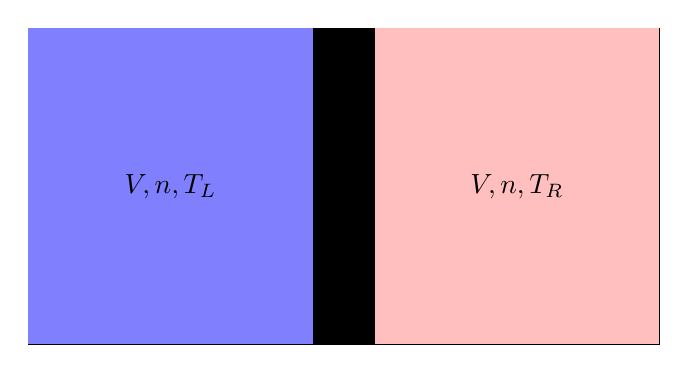
\begin{tikzpicture}[scale=4]
        \draw[black, thick] (0,0) rectangle (2,1);
        \filldraw[fill = black, draw = black] (0.9,0) rectangle (1.1,1);
        \filldraw[fill = blue!50, draw = blue!50] (0,0) rectangle(0.9,1);
         \filldraw[fill = pink, draw = pink] (1.1,0) rectangle(2,1);
        \draw[black] (0.45,0.5) node {$V,n,T_L$};
        \draw[black] (1.55,0.5) node {$V,n,T_R$};
        
        \end{tikzpicture}
    \end{center}
\end{enumerate}
\newpage
\section{Solutions to Practice Problems}
\subsection{Temperature and Other Fundamentals Solutions}
\begin{enumerate}
    \item Particles in an ideal gas undergo elastic collisions. It is one of the necessary conditions for a gas to be considered ideal.
    \item \begin{enumerate}
        \item Substituting $k_b = \frac{R}{N_A}$ into the ideal gas law $PV = Nk_bT$, we get:
    \[PV = N\frac{R}{N_A}T \]
    And the number of molecules $N$ divided by Avogadro's number is just the number of moles of gas $n$, so this becomes:
    \[PV = nRT \]
    As desired.
        \item This answer follows a very similar process to the previous problem. Substituting $k_b = \frac{R}{N_A}$ into the thermal energy of the system $E_{th} = \frac{\chi}{2}Nk_bT$, we get:
    \[ E_{th} = \frac{\chi}{2}N\frac{R}{N_A}T \]
    And using the same identity of $\frac{N}{N_A} = n$, as above:
    \[ E_{th} = \frac{\chi}{2}nRT \]
    As desired.
        \item ubstituting $PV = nRT$ into $E_{th} = \frac{\chi}{2}nRT$, we obtain:
    \[ E_{th} = \frac{\chi}{2}PV \]
    As desired. 
    \end{enumerate}
    \item No, two systems having the same amount of total energy does not imply the same amount of temperature. Temperature is a measure of the average kinetic energy of particles, while total thermal energy is the measure of \textbf{all} the thermal energy of all the particles in the system. For example, a large ice cube and a millilitre of boiling water could have the same thermal energy, but clearly are at different temperatures. Mathematically, one only needs to look at the equation \[ E_{th} = \frac{\chi}{2}nRT \] to see that thermal energy depends not only on temperature, but the amount of stuff that you have (As well as the degrees of freedom of the stuff). 
    \item Assuming that this vacuum-box is placed in a room with any molecules, then no. A vacuum is the absence of molecules, and in the absence of any molecules, you don't have any pressure on the walls of the box. So the inside of the box will have a different pressure than the outside, and hence not be in equilibrium.
    \item \begin{enumerate}
        \item If the volume of a box of ideal box decreased, then $V$ would decrease, while
        the amount of gas $n$ and the temperature of gas $T$ would stay the same (as the average kinetic energy of the molecules wouldn't change in this case). Therefore by the ideal gas law $PV = nRT$, if the right hand side stays the same size while $V$ decreases, then the pressure $P$ must increase.
        \item By the same logic as above, if the volume of the box of ideal gas increased, the pressure $P$ must decrease.
        \item If the box of ideal gas springs a leak, then the amount of gas $n$ in the box decreases, while the volume $V$ and the temperature $T$ of the box would stay the same (as again, the average kinetic energy of the particles would not be affected). Therefore, by the ideal gas law $PV = nRT$, the pressure $P$ must decrease (as we would expect from any container that sprung a leak!)
    \end{enumerate}
    \item If this hypothetical super-heavy gas indeed could exist, then it clearly couldn't be ideal, as the gravitational attraction between the gas particles would be significant. So this isn't a situation where we can apply the ideal gas law. However, principles of energy conservation would still apply (as they always do). When we increase the volume of the box, the average distance between any two superheavy molecules will increase. When we increase the distance between the super-heavy gas molecules, the gravitational potential energy $U_g = -\frac{GM^2}{r}$ (Where $G$ is the gravitational constant, $m$ is the mass of one super-heavy molecule, and $r$ is the distance in between two molecules) increases (or to be more clear, it becomes less negative, as $r$ increases). Therefore, if the potential energy increases, energy conservation tells us that kinetic energy must then decrease. Another way of thinking about this is to pull appart two massive objects, I need to put energy into the system to pull them apart; this energy comes from the kinetic energy of the molecules in this case. Either way, the decrease of the kinetic energy of molecules means that by our definition of temperature $T=\frac{2}{3 k_{b}} \epsilon_{kavg}$ which linearly scales with the kinetic energy, the temperature of the super-heavy molecules must decrease. 
    \item This question follows a similar thought process to the one above. Since we have a gas of electrons which clearly would interact with one another through the electrostatic force, our gas again is not ideal. However, we once again consider an argument from energy conservation. This time, the electric potential energy between two negatively charged electrons is given by $U_{q} = \frac{ke^2}{r}$, where $k$ is the constant in Coloumb's law, $e$ is the elementary charge on the electron, and $r$ is the distance between any two electrons. In this case, increasing the volume of the box and increasing the average distance between two electrons will lead to a decrease in the electric potential energy. Therefore, by energy conservation, the kinetic energy of the electrons must increase, and we would then have that the temperature of the electron gas would increase by the definition.
    \item \begin{enumerate}
        \item By equation \ref{eqn:(2)} of $\frac{3}{2}PV = N\epsilon_{kavg}$ we see that the pressure of of the box scales linearly with the number of particles. Therefore, the box with the greater number of particles would have greater pressure. However, temperature is independent of the number of particles, (as it only depends on the average kinetic energy of all the particles, by the definition $T=\frac{2}{3 k_{b}} \epsilon_{kavg}$) so therefore the temperature of the two boxes would be the same.  
        \item Again looking at equation \ref{eqn:(2)} of $\frac{3}{2}PV = N\epsilon_{kavg}$, we see that the pressure scales linearly with kinetic energy; kinetic energy is linear in the mass $m$ of the particles. Therefore, the
        box with the heavier (but identical speed) molecules would have greater kinetic energy and therefore greater pressure. By the same argument, since temperature also scales linearly with kinetic energy, the heavier-particle box would also have a higher temperature.
    \end{enumerate}
    \item I would have to supply three times as much heat. Recalling equation \ref{eqn:(13)} which relates the energy change with temperature, we have:
    \begin{align*}
        \Delta E = nc_v\Delta T = n\frac{\chi}{2}\Delta T
    \end{align*}
    Where $\Delta E$ is the change in temperature, $n$ is the number of moles of gas, $\chi$ is the degrees of freedom of the molecule. and $\Delta T$ is the change in temperature. For a monoatomic molecule, we have $\chi = 3$ and for a triatomic molecule, we have $\chi=6$. Therefore, per unit of temperature change, we would require three times as much energy for the triatomic 
    \item A monoatomic molecule in 10 dimensional space would still not have any rotational degrees of freedom, but would have 10 translational degrees of freedom (don't bother thinking about what this looks like...) By the same argument given in the previous section, since the 10-D helium has more degrees of freedom, it would have a smaller temperature increase than the 3-D helium if both were given the same amount of energy. 
\end{enumerate}
\subsection{\texorpdfstring{The 1\textsuperscript{st} Law of Thermodynamics Solutions}{The 1st Law of Thermodynamics Solutions}}
\begin{enumerate}
    \item 
    \begin{enumerate} 
    \item Rearranging equation \ref{eqn:(33)}, to solve for pressure, we have:
    \begin{gather*}
        \left(P+a\frac{n^2}{V^2}\right)V = nRT \\
        PV + a\frac{n^2}{V} = nRT \\
        PV = nRT - \frac{an^2}{V} \\
        P = \frac{nRT}{V}-\frac{an^2}{V^2}
    \end{gather*}
    \item Applying equation \ref{eqn:(16)} (the equation for thermodynamic work), we have:
    \[W = -\int_{V_1}^{V_2}P(V)dV = -\int_{V_1}^{V_2}\left(\frac{nRT}{V}-\frac{an^2}{V^2} \right)dV \]
    \end{enumerate}
    As the compression is isothermal, $T$ is constant and I can take it out of the integral. The remaining integrals for $V$ are elementary:
    \[W = an^2\int_{V_1}^{V_2}\frac{1}{V^2}dV - nRT\int_{V_1}^{V_2}\frac{1}{V}dV \]
    \[ W = an^2 \left. -\frac{1}{V}\right|_{V_1}^{V_2} + nRT\left. \ln(V)\right|_{V_1}^{V_2} \]
    \[W = an^2\left(\frac{1}{V_1}-\frac{1}{V_2}\right) + nRT\ln\left(\frac{V_2}{V_1}\right)\]
    So we see that the work done is very similar to the ideal gas isothermal compression, just with an additional corrective term of $an^2\left(\frac{1}{V_1}-\frac{1}{V_2}\right)$.
    \item Answers summarized in chart below. Note that we define all the signs here in terms of what is done to the gas. So, + work done on gas is when we do work, - work done on gas is when the gas does work for us. + Heat flow into the gas means we supply heat to the gas, - heat flow into the gas means the gas releases heat.
\begin{center}
 \begin{tabular}{|c| c | c | c|} 
 \hline
 \textbf{Process} & \textbf{Work on gas} & \textbf{Heat into gas} & $\Delta T$\\ 
 \hline\hline
 Isochoric heating & 0 & + & + \\
 Isochoric cooling & 0 & - & - \\
 Isobaric expansion & - & + & + \\
 Isobaric compression & + & - & - \\
 Isothermal expansion & - & + & 0 \\
 Isothermal compression & + & - & 0 \\
 Adiabatic expansion & - & 0 & - \\
 Adiabatic compression & + & 0 & + \\
 \hline
 \end{tabular}
 \end{center}
    \item 
    \begin{enumerate}
        \item Internal energy is a function of state, and after one cycle the system is back in its initial state. Therefore, the net change in internal energy is zero.
        \item There's an easy way to do this; just calculate the area of the triangle in the graph. So
        \begin{align*}
            W_{net} &= \frac{2\textrm{m}^3\cdot 10\textrm{kPa}}{2}
            = 10\textrm{kJ}
        \end{align*}
        So the work done by the engine in one cycle is $10\textrm{kJ}$. 
        \item Since the net change in internal energy of the heat engine is zero, and the heat engine does $10\textrm{kJ}$ of work per cycle, by the first law of thermodynamics, there must be a net flow of $10\textrm{kJ}$ of heat \textit{into} the engine per cycle.
        \item From ideal gas law, we know that $T = \frac{PV}{nR}$. We know that $n=1\textrm{mol}$, and we can just plug in the known values of $P$ and $V$ at each point. For $1$, we have $P = 5\textrm{kPa}, V = 4\textrm{m}^3$, so $T_1 = \frac{5000\textrm{Pa}*4\textrm{m}^3}{1\textrm{mol}*8.314\textrm{ J} \textrm{ mol}^{-1} \textrm{ K}^{-1}} \approx 2,406 \textrm{K}$. Similarly, for $2$ we have $P = 5\textrm{kPa}, V = 2\textrm{m}^3$, giving us $T_2 \approx 1203\textrm{K}$, and for $3$ we have $P = 15\textrm{kPa}, V = 2\textrm{m}^3$, giving us $T_3 \approx 3608\textrm{K}$. This is perhaps an unrealistically hot engine!
        \item Starting with work, we already know that the cycle does a net work of 10kJ on the environment. In process $1 \rightarrow 2$, we can calculate the area under the graph (a nice easy rectangle) to get that the gas does $W = -10\textrm{kJ}$, or we do $10\textrm{kJ}$ of work on the gas. Since process $2 \rightarrow 3$ is isochoric, no work is done. Finally, we can see on the graph that the work done by $3 \rightarrow 1$ is the area of the triangle plus the area of the rectangle. So, this process does $20\textrm{kJ}$ of work on the environment. Adding up the work done during each process, we recover the original net work value of $10\textrm{kJ}$ that the engine does for us. \\
        Now to solve for the heat. For process $1 \rightarrow 2$, we have that $Q = -nc_p\Delta T$ (as we derived for an isobaric process) where $c_p = \frac{\chi}{2}R+R = \frac{5}{2}R$ for a monoatomic gas, and $\Delta T = T_2-T_1 = 2406\mathrm{K} -1203\mathrm{K}  = 1203\mathrm{K} $. Therefore, we have that:
        \[Q_{1\rightarrow 2} = nc_p\Delta T = 1\textrm{mol}*\frac{5}{2}*8.314\textrm{ J} \textrm{ mol}^{-1} \textrm{K}^{-1}*1203\mathrm{K} \approx 25\textrm{kJ}\]
        So we find that 25kJ of heat leaves the engine. \\
        For process $2\rightarrow 3$, we have an isochoric process, so $Q = nc_v\Delta T$, where $c_v = \frac{3}{2}R$ and $\Delta T = T_3-T_2 = 3608\textrm{K}-1202\textrm{K} = 2406\textrm{K}$, so we have that:
        \[Q_{2\rightarrow 3} = nc_v\Delta T = 1\textrm{mol}*\frac{3}{2}*8.314\textrm{ J} \textrm{ mol}^{-1} \textrm{K}^{-1}*2406\mathrm{K} \approx 30\textrm{kJ}\]
        So we find that 30kJ of heat enters the engine. \\
        Finally, for process $3 \rightarrow 1$, we have a bit of a strange process that we haven't defined and doesn't follow a nice rule of something being held constant. In this case, we use the first law of thermodynamics:
        \[ \Delta E = Q+W \]
        and combine it with the relation:
        \[ \Delta E = nc_v\Delta T \]
        To get:
        \[nc_v\Delta T = Q+W\]
        We know that $W = -20\textrm{kJ}$ in this process from the area underneath the curve (the gas does 20kJ of work), and we can solve for $\Delta T = T_1-T_3 = 2406\textrm{K}-3608\textrm{K} = -1,202\textrm{K}$. Plugging everything in, we find:
        \[Q = 1\textrm{mol}*\frac{3}{2}*8.314\textrm{ J} \textrm{ mol}^{-1} \textrm{K}^{-1}*-1202\mathrm{K} + 20\textrm{kJ} \approx 5\textrm{kJ}\]
        So we obtain that 5kJ of heat flows into the engine during this process.
    \end{enumerate}
    \item
    \begin{enumerate}
        \item Since process $3 \rightarrow 1$ is isothermal, $T_1 = T_3$. So, the ratio would be 1:1.
        \item Since $3 \rightarrow 1$ is an isothermal process, we have that $P_1V_1 = P_3V_3$. This can then be rearranged to get that $P_3 = 2P_0$.
        \item Using the same method as in 3) we can see from the graph that point 2 has the lowest temperature. Since $3 \rightarrow 1$ is isothermal, that means that points 3, 1, and any point on the process between are at the highest temperature.
        \item We'll start off by calculating the heat flowing into the engine. Heat must flow into the engine during processes $2 \rightarrow 3$ (since it gains energy with no work done) and $3 \rightarrow 1$ (since it does work but remains at the same energy). Since $2 \rightarrow 3$ is isochoric we can say that
        \begin{align*}
            Q &= \Delta E \\
            &= nc_V\Delta T \\
            &= nc_V\Delta\frac{PV}{nR} \text{  applying ideal gas law} \\
            &= \frac{\chi}{2}V_2(P_3 - P_2) \\
            &= \frac{\chi}{2}\frac{V_0}{2}(2P_0 - P_0) \\
            &= \frac{\chi}{4}V_0P_0
        \end{align*}
        Next, since process $3 \rightarrow 1$ is isothermal we can say that
        \begin{align*}
            Q &= -W \\
            &= -nRT\ln{\frac{V_3}{V_1}} \\
            &= nR\frac{P_1V_1}{nR}\ln{\frac{V_1}{V_3}} \\
            &= P_0V_0\ln{\frac{V_0}{V_0/2}} \\
            &= P_0V_0\ln{2}
        \end{align*}
        So in total we get that $Q_{in} = \frac{\chi}{4}V_0P_0 + P_0V_0\ln{2}$. Next, we'll deal with the net work done by the system. Process $1 \rightarrow 2$ is isobaric, so we can pretty quickly calculate that we do $\frac{P_0V_0}{2}$ joules of work on the system. Process $2 \rightarrow 3$ is isochoric and does no work. Since process $3 \rightarrow 1$ is isothermal, we can say that $W = -Q$. Thus, we get that $P_0V_0\ln{2}$ joules of work is done on the environment. Combining these together to calculate efficiency we get
        \begin{align*}
            \eta &= \frac{W_{net}}{Q_{in}} \\
            &= \frac{P_0V_0\ln{2} - \frac{P_0V_0}{2}}{\frac{\chi}{4}V_0P_0 + P_0V_0\ln{2}} \\
            &= \frac{\ln{2} - \frac{1}{2}}{\frac{\chi}{4} + \ln(2)}
        \end{align*}
        For any monoatomic gas, $\chi = 3$, so we get that $\eta \approx 0.13$.
    \end{enumerate}
    \item 
    \begin{enumerate}
        \item The quickest way way to solve it is with process $3 \rightarrow 1$ (although you could also use all three processes, if you so desired). Since this process is adiabatic, we have that
        \begin{gather*}
            T_1V_1^{\gamma-1} = T_3V_3^{\gamma-1} \\
            \frac{T_3}{T_1} = \frac{V_1}{V_3}^{\gamma-1}
        \end{gather*}
        For monoatomic gasses, $\gamma = \frac{5}{3}$ so plugging in all the values
        \begin{equation*}
            \frac{T_3}{T_1} = \frac{V_0}{V_0/2}^{\frac{2}{3}} \\
            \frac{T_3}{T_1} = 2^{\frac{2}{3}}
        \end{equation*}
        \item We're basically doing the same thing here. We can say that 
        \begin{gather*}
            P_1V_1^{\gamma} = P_3V_3^{\gamma} \\
            P_3 = P_1\frac{V_1}{V_3}^{\gamma} \\
            P_3 = P_1\frac{V_1}{V_3}^{\frac{5}{3}} \\
            P_3 = P_0 2^{\frac{5}{3}}
        \end{gather*}
        \item Using the same logic as we did for question 3, it's pretty clear on the graph that point 2 has the lowest temperature. We also know from a) that $\frac{T_3}{T_1} > 1$, so we get that point 3 has the highest temperature.
        \item Let's start with the net heat put into the system. Heat only flows into the system in process $2 \rightarrow 3$, so we'll focus on that. In this process no work is done, so we get that $Q = nc_V\Delta T$. The problem is we don't know the temperature in either state. However, we can get tricky with this to rearrange into something more manageable using ideal gas law and the previous parts of this question
        \begin{align*}
            Q &= nc_V(\frac{V_2\Delta P}{nR}) \text{  from ideal gas law} \\
            &= \frac{\chi}{2}V_2\Delta P \\
            &= \frac{\chi}{2}V_2(P_3 - P_2) \\
            &= \frac{\chi}{2}(V_0\cdot 2^{-1})(P_0\cdot 2^{\frac{5}{3}} - P_0\cdot 2^{-1}) \text{  from part b} \\
            &= \frac{\chi}{4}V_0P_0(2^{\frac{8}{3}} - 1)
        \end{align*}
        Ouch. Well no matter, we soldier on to work which is going to be even more difficult. Fun. Let's start with the easy part. Work is only done on the system during process $1 \rightarrow 2$. Since its an isobaric process, this leads us to conclude that $W_{1\rightarrow 2} = \frac{P_0V_0}{2}$. Nice! Now for process $2 \rightarrow 3$, where the system does work (much less nice). We're going to use a similar trick to last time, except our expression for work is coming from adiabatic processes (the negative is placed in front because work on the surroundings is normally considered negative)
        \begin{gather*}
            \Delta E = -W \\
            W = -nC_V\Delta T \\
            W = -nc_V(\frac{\Delta VP}{nR}) \text{  from ideal gas law} \\
            W = -\frac{\chi}{2}(P_1V_1 - P_3V_3) \\
            W = \frac{\chi}{2}(P_0\frac{V_0}{2}2^{\frac{5}{3}} - P_0V_0) \\
            W = \frac{\chi}{2}P_0V_0(2^{\frac{2}{3}} - 1)
        \end{gather*}
        And yet another ooof done. So, we now get that the net work is
        \begin{align*}
            W_{net} &= \frac{\chi}{2}P_0V_0(2^{\frac{2}{3}} - 1) - \frac{P_0V_0}{2} \\
            &= \frac{P_0V_0}{2}(\chi(2^{\frac{2}{3}} - 1) - 1)
        \end{align*}
        We're almost there! Now all that remains is to plug these into the efficiency equation
        \begin{align*}
            \eta &= \frac{W_{net}}{Q_{in}} \\
            &= \frac{\frac{P_0V_0}{2}(\chi(2^{\frac{2}{3}} - 1) - 1)}{\frac{\chi}{4}V_0P_0(2^{\frac{8}{3}} - 1)} \\
            &= 2\frac{\chi(2^{\frac{2}{3}} - 1) - 1}{\chi(2^{\frac{8}{3}} - 1)}
        \end{align*}
        For a monoatomic gas, $\chi = 3$ so we get that $\eta \approx 0.095$. All that for a less efficient process!
    \end{enumerate}
    An interesting thing to note is that the heat engine in 4) is more efficient than the one in 5) only for monoatomic gases. This is of course assuming that diatomic and triatomic gases follow ideal gas law, which isn't a bad approximation (for "low" pressures).
    \item As a quick reminder, we're trying to prove that $\frac{V_2}{V_1} = \frac{V_3}{V_4}$ in our Carnot engine. Since the processes from states d to a and b to c are adiabatic, we have that
    \begin{equation*}
        P_1V_1^\gamma = P_4V_4^\gamma \hspace{2cm} P_2V_2^\gamma = P_3V_3^\gamma
    \end{equation*}
    Since the processes from states a to b and c to d are isothermal, we have that
    \begin{equation*}
        P_1V_1 = P_2V_2 \hspace{2cm} P_3V_3 = P_4V_4
    \end{equation*}
    Since the pressure and volume are both nonzero, we can divide the first two equations to get
    \begin{equation*}
        \frac{P_1V_1^\gamma}{P_2V_2^\gamma} = \frac{P_4V_4^\gamma}{P_3V_3^\gamma}
    \end{equation*}
    Which we can factor to
    \begin{equation*}
        \frac{P_1V_1V_1^{\gamma - 1}}{P_2V_2V_2^{\gamma - 1}} = \frac{P_4V_4V_4^{\gamma - 1}}{P_3V_3V_3^{\gamma - 1}}
    \end{equation*}
    Which, by the third and fourth equations we can see is equivalent to
    \begin{equation*}
        \frac{V_1^{\gamma - 1}}{V_2^{\gamma - 1}} = \frac{V_4^{\gamma - 1}}{V_3^{\gamma - 1}}
    \end{equation*}
    We know that $\gamma > 1$, so we can take the $(\gamma - 1)$th root of both sides to get
    \begin{equation*}
        \frac{V_1}{V_2} = \frac{V_4}{V_3}
    \end{equation*}
    Or, inverting the equation
    \begin{equation*}
        \frac{V_2}{V_1} = \frac{V_3}{V_4}
    \end{equation*}
\end{enumerate}
\subsection{Entropy Solutions}
\begin{enumerate}
    \item For any process, we define the change in entropy as the sum of $\frac{\delta Q}{T}$ for many infinitesimal steps. In an adiabatic process, heat never flows, so $\delta Q = 0$ for all of these steps. Thus, in an adiabatic process the entropy of a system remains constant.
    \item There are four triplets of numbers that could sum to $7$, $(5,1,1)$, $(4,2,1)$, $(3,3,1)$, and $(3,2,2)$. Each of these has $3!$ orders they could be rolled in. Hence there are $24$ microstates, for a total entropy of $k_{b}\ln{24}$.
    \item In this case, all possible orders of those four triples are considered the same microstate. So we instead have four possible microstates, for a total entropy of $k_{b}\ln{4}$.
    \item After one cycle, the gas medium of a heat engine is in its initial state. Since entropy is a function of state, the gas must then have the same total entropy as it did at the start of a cycle. So after one cycle, the gas's entropy will not change.
    \item The number of possible ways that the particles could be distributed after removing the partition is much higher than before the partition was removed (i.e. the disorder of the system increases quite a bit). So, the entropy of the system has increased. Therefore, to spontaneously return to their initial state the gases would have to violate the second law of thermodynamics. (One thing to note here is that it's technically possible that the system will eventually momentarily reach its original configuration, just extremely unlikely).
    \item Using the Sackur-Tetrode equation we have that 
    \begin{equation*}
        \Delta S = nc_{v}\ln{\frac{T_1}{T_0}} + nR\ln{\frac{V_1}{V_0}}.
    \end{equation*}
    $T_0 = 300\textrm{K}$, $T_1 = 400\textrm{K}$, and $n = 1\textrm{mol}$ are given. Furthermore, since it expands to double its original size, we know that $V_1 = 2V_0$. Finally, we know that the gas has 3 degrees of freedom, since its monoatomic, and therefore $c_v = \frac{3}{2}R$. So plugging those in we get
    \begin{gather*}
        \Delta S = (1\textrm{mol})(\frac{3}{2})(8.314\frac{\textrm{J}}{\textrm{mol}\cdot \textrm{K}})\ln{\frac{400\textrm{K}}{300\textrm{K}}} + (1\textrm{mol})(8.314\frac{\textrm{J}}{\textrm{mol}\cdot \textrm{K}})\ln{\frac{2V_0}{V_0}} \\
        \Delta S \approx 9.35\frac{\textrm{J}}{\textrm{K}}
    \end{gather*}
    \item
    \begin{enumerate}
        \item From the ideal gas law, if both compartments have the same amount and volume of gas, but the right side has a higher temperature, then we know that the right side will have a higher pressure than the left. Therefore, the gas on the right side will expand and the gas on the left side of the box will be compressed (as the gas molecules on the right are pushing with more force on the central piston), in an adiabatic process (as no heat can flow). The process will terminate once the pressure on both sides of the box is equal.
        \item Since this process resulted in no energy gain or loss (as the box is isolated from its environment), the internal energy change of the system is zero. Since this process raises the temperature on the left to be closer to that on the right, you would think that this process raises the entropy of the system. However, since both sides of the box underwent an adiabatic process, neither had a change in entropy. Entropy is an extensive quantity, so the entropy of the box must have remained constant as well.
        \item At the end, the pressure of the two sides would be equal, as the net force on the central piston would be zero. The volume of the left side would be less than the right. Finally, since both sides of the box have the same number of moles of gas, we can use ideal gas law to say that after the process is over:
    \[
        \frac{P_lV_l}{T_l} = \frac{P_rV_r}{T_r}
    \]
    which since the final pressures are equal simplifies to
    \[
        \frac{V_l}{T_l} = \frac{V_r}{T_r}
    \]
    We know that the final volume of the left side is less than the final volume on the right side. Therefore, the final temperature on the right must be greater than that on the left. The system is not in thermal equilibrium, which does make sense as the two containers were not in thermal contact with one another.
    \end{enumerate}   
\end{enumerate}

\end{document}
